\documentclass[a4paper]{article}

\def\npart {II}
\def\nterm {Lent}
\def\nyear {2015}
\def\nlecturer {I. B. Leader}
\def\ncourse {Logic and Set Theory}

% Imports
\ifx \nextra \undefined
  \usepackage[pdftex,
    hidelinks,
    pdfauthor={Dexter Chua},
    pdfsubject={Cambridge Maths Notes: Part \npart\ - \ncourse},
    pdftitle={Part \npart\ - \ncourse},
  pdfkeywords={Cambridge Mathematics Maths Math \npart\ \nterm\ \nyear\ \ncourse}]{hyperref}
  \title{Part \npart\ - \ncourse}
\else
  \usepackage[pdftex,
    hidelinks,
    pdfauthor={Dexter Chua},
    pdfsubject={Cambridge Maths Notes: Part \npart\ - \ncourse\ (\nextra)},
    pdftitle={Part \npart\ - \ncourse\ (\nextra)},
  pdfkeywords={Cambridge Mathematics Maths Math \npart\ \nterm\ \nyear\ \ncourse\ \nextra}]{hyperref}

  \title{Part \npart\ - \ncourse \\ {\Large \nextra}}
\fi

\author{Lectured by \nlecturer \\\small Notes taken by Dexter Chua}
\date{\nterm\ \nyear}

\usepackage{alltt}
\usepackage{amsfonts}
\usepackage{amsmath}
\usepackage{amssymb}
\usepackage{amsthm}
\usepackage{booktabs}
\usepackage{caption}
\usepackage{enumitem}
\usepackage{fancyhdr}
\usepackage{graphicx}
\usepackage{mathtools}
\usepackage{microtype}
\usepackage{multirow}
\usepackage{pdflscape}
\usepackage{pgfplots}
\usepackage{siunitx}
\usepackage{tabularx}
\usepackage{tikz}
\usepackage{tkz-euclide}
\usepackage[normalem]{ulem}
\usepackage[all]{xy}

\pgfplotsset{compat=1.12}

\pagestyle{fancyplain}
\lhead{\emph{\nouppercase{\leftmark}}}
\ifx \nextra \undefined
  \rhead{
    \ifnum\thepage=1
    \else
      \npart\ \ncourse
    \fi}
\else
  \rhead{
    \ifnum\thepage=1
    \else
      \npart\ \ncourse\ (\nextra)
    \fi}
\fi
\usetikzlibrary{arrows}
\usetikzlibrary{decorations.markings}
\usetikzlibrary{decorations.pathmorphing}
\usetikzlibrary{positioning}
\usetikzlibrary{fadings}
\usetikzlibrary{intersections}
\usetikzlibrary{cd}

\newcommand*{\Cdot}{\raisebox{-0.25ex}{\scalebox{1.5}{$\cdot$}}}
\newcommand {\pd}[2][ ]{
  \ifx #1 { }
    \frac{\partial}{\partial #2}
  \else
    \frac{\partial^{#1}}{\partial #2^{#1}}
  \fi
}

% Theorems
\theoremstyle{definition}
\newtheorem*{aim}{Aim}
\newtheorem*{axiom}{Axiom}
\newtheorem*{claim}{Claim}
\newtheorem*{cor}{Corollary}
\newtheorem*{defi}{Definition}
\newtheorem*{eg}{Example}
\newtheorem*{fact}{Fact}
\newtheorem*{law}{Law}
\newtheorem*{lemma}{Lemma}
\newtheorem*{notation}{Notation}
\newtheorem*{prop}{Proposition}
\newtheorem*{thm}{Theorem}

\renewcommand{\labelitemi}{--}
\renewcommand{\labelitemii}{$\circ$}
\renewcommand{\labelenumi}{(\roman{*})}

\let\stdsection\section
\renewcommand\section{\newpage\stdsection}

% Strike through
\def\st{\bgroup \ULdepth=-.55ex \ULset}

% Maths symbols
\newcommand{\bra}{\langle}
\newcommand{\ket}{\rangle}

\newcommand{\N}{\mathbb{N}}
\newcommand{\Z}{\mathbb{Z}}
\newcommand{\Q}{\mathbb{Q}}
\renewcommand{\H}{\mathbb{H}}
\newcommand{\R}{\mathbb{R}}
\newcommand{\C}{\mathbb{C}}
\newcommand{\Prob}{\mathbb{P}}
\renewcommand{\P}{\mathbb{P}}
\newcommand{\E}{\mathbb{E}}
\newcommand{\F}{\mathbb{F}}
\newcommand{\cU}{\mathcal{U}}
\newcommand{\RP}{\mathbb{RP}}
\newcommand{\CP}{\mathbb{CP}}

\newcommand{\ph}{\,\cdot\,}

\DeclareMathOperator{\sech}{sech}
\DeclareMathOperator{\cosech}{cosech}
\DeclareMathOperator{\cosec}{cosec}

\DeclareMathOperator{\covol}{covol}
\DeclareMathOperator{\vol}{vol}

\let\Im\relax
\let\Re\relax
\DeclareMathOperator{\Im}{Im}
\DeclareMathOperator{\Re}{Re}
\DeclareMathOperator{\im}{im}
\DeclareMathOperator{\image}{image}
\DeclareMathOperator{\Ann}{Ann}

\DeclareMathOperator*{\res}{res}
\DeclareMathOperator{\Res}{Res}
\DeclareMathOperator{\Ind}{Ind}

\DeclareMathOperator{\tr}{tr}
\DeclareMathOperator{\diag}{diag}
\DeclareMathOperator{\rank}{rank}
\DeclareMathOperator{\card}{card}
\DeclareMathOperator{\spn}{span}
\DeclareMathOperator{\adj}{adj}

\DeclareMathOperator{\erf}{erf}
\DeclareMathOperator{\erfc}{erfc}

\DeclareMathOperator{\ord}{ord}
\DeclareMathOperator{\Sym}{Sym}

\DeclareMathOperator{\sgn}{sgn}
\DeclareMathOperator{\orb}{orb}
\DeclareMathOperator{\stab}{stab}
\DeclareMathOperator{\ccl}{ccl}

\DeclareMathOperator{\lcm}{lcm}
\DeclareMathOperator{\hcf}{hcf}

\DeclareMathOperator{\Int}{Int}
\DeclareMathOperator{\id}{id}

\DeclareMathOperator{\betaD}{beta}
\DeclareMathOperator{\gammaD}{gamma}
\DeclareMathOperator{\Poisson}{Poisson}
\DeclareMathOperator{\binomial}{binomial}
\DeclareMathOperator{\multinomial}{multinomial}
\DeclareMathOperator{\Bernoulli}{Bernoulli}
\DeclareMathOperator{\like}{like}

\DeclareMathOperator{\var}{var}
\DeclareMathOperator{\cov}{cov}
\DeclareMathOperator{\bias}{bias}
\DeclareMathOperator{\mse}{mse}
\DeclareMathOperator{\corr}{corr}

\DeclareMathOperator{\otp}{otp}
\DeclareMathOperator{\dom}{dom}

\DeclareMathOperator{\Root}{Root}
\DeclareMathOperator{\supp}{supp}
\DeclareMathOperator{\rel}{rel}
\DeclareMathOperator{\Hom}{Hom}
\DeclareMathOperator{\Aut}{Aut}
\DeclareMathOperator{\Gal}{Gal}
\DeclareMathOperator{\Mat}{Mat}
\DeclareMathOperator{\End}{End}
\DeclareMathOperator{\Char}{char}
\DeclareMathOperator{\ev}{ev}
\DeclareMathOperator{\St}{St}
\DeclareMathOperator{\Lk}{Lk}
\DeclareMathOperator{\disc}{disc}
\DeclareMathOperator{\Isom}{Isom}
\DeclareMathOperator{\length}{length}
\DeclareMathOperator{\energy}{energy}
\DeclareMathOperator{\area}{area}
\DeclareMathOperator{\Syl}{Syl}
\DeclareMathOperator{\cl}{cl}
\DeclareMathOperator{\fix}{fix}

\newcommand{\GL}{\mathrm{GL}}
\newcommand{\SL}{\mathrm{SL}}
\newcommand{\PGL}{\mathrm{PGL}}
\newcommand{\PSL}{\mathrm{PSL}}
\newcommand{\PSU}{\mathrm{PSU}}
\newcommand{\Or}{\mathrm{O}}
\newcommand{\SO}{\mathrm{SO}}
\newcommand{\U}{\mathrm{U}}
\newcommand{\SU}{\mathrm{SU}}

\renewcommand{\d}{\mathrm{d}}
\newcommand{\D}{\mathrm{D}}

\tikzset{->/.style = {decoration={markings,
                                  mark=at position 1 with {\arrow[scale=2]{latex'}}},
                      postaction={decorate}}}
\tikzset{<-/.style = {decoration={markings,
                                  mark=at position 0 with {\arrowreversed[scale=2]{latex'}}},
                      postaction={decorate}}}
\tikzset{<->/.style = {decoration={markings,
                                   mark=at position 0 with {\arrowreversed[scale=2]{latex'}},
                                   mark=at position 1 with {\arrow[scale=2]{latex'}}},
                       postaction={decorate}}}
\tikzset{->-/.style = {decoration={markings,
                                   mark=at position #1 with {\arrow[scale=2]{latex'}}},
                       postaction={decorate}}}
\tikzset{-<-/.style = {decoration={markings,
                                   mark=at position #1 with {\arrowreversed[scale=2]{latex'}}},
                       postaction={decorate}}}

\tikzset{circ/.style = {fill, circle, inner sep = 0, minimum size = 3}}
\tikzset{mstate/.style={circle, draw, blue, text=black, minimum width=0.7cm}}

\definecolor{mblue}{rgb}{0.2, 0.3, 0.8}
\definecolor{morange}{rgb}{1, 0.5, 0}
\definecolor{mgreen}{rgb}{0.1, 0.4, 0.2}
\definecolor{mred}{rgb}{0.5, 0, 0}

\def\drawcirculararc(#1,#2)(#3,#4)(#5,#6){%
    \pgfmathsetmacro\cA{(#1*#1+#2*#2-#3*#3-#4*#4)/2}%
    \pgfmathsetmacro\cB{(#1*#1+#2*#2-#5*#5-#6*#6)/2}%
    \pgfmathsetmacro\cy{(\cB*(#1-#3)-\cA*(#1-#5))/%
                        ((#2-#6)*(#1-#3)-(#2-#4)*(#1-#5))}%
    \pgfmathsetmacro\cx{(\cA-\cy*(#2-#4))/(#1-#3)}%
    \pgfmathsetmacro\cr{sqrt((#1-\cx)*(#1-\cx)+(#2-\cy)*(#2-\cy))}%
    \pgfmathsetmacro\cA{atan2(#2-\cy,#1-\cx)}%
    \pgfmathsetmacro\cB{atan2(#6-\cy,#5-\cx)}%
    \pgfmathparse{\cB<\cA}%
    \ifnum\pgfmathresult=1
        \pgfmathsetmacro\cB{\cB+360}%
    \fi
    \draw (#1,#2) arc (\cA:\cB:\cr);%
}
\newcommand\getCoord[3]{\newdimen{#1}\newdimen{#2}\pgfextractx{#1}{\pgfpointanchor{#3}{center}}\pgfextracty{#2}{\pgfpointanchor{#3}{center}}}

\def\Xint#1{\mathchoice
   {\XXint\displaystyle\textstyle{#1}}%
   {\XXint\textstyle\scriptstyle{#1}}%
   {\XXint\scriptstyle\scriptscriptstyle{#1}}%
   {\XXint\scriptscriptstyle\scriptscriptstyle{#1}}%
   \!\int}
\def\XXint#1#2#3{{\setbox0=\hbox{$#1{#2#3}{\int}$}
     \vcenter{\hbox{$#2#3$}}\kern-.5\wd0}}
\def\ddashint{\Xint=}
\def\dashint{\Xint-}


\begin{document}
\maketitle
{\small
  \noindent\textbf{Ordinals and cardinals}\\
  Well-orderings and order-types. Examples of countable ordinals. Uncountable ordinals and Hartogs' lemma. Induction and recursion for ordinals. Ordinal arithmetic. Cardinals; the hierarchy of alephs. Cardinal arithmetic.\hspace*{\fill} [5]

  \vspace{10pt}
  \noindent\textbf{Posets and Zorn's lemma}\\
  Partially ordered sets; Hasse diagrams, chains, maximal elements. Lattices and Boolean algebras. Complete and chain-complete posets; fixed-point theorems. The axiom of choice and Zorn's lemma. Applications of Zorn's lemma in mathematics. The well-ordering principle.\hspace*{\fill} [5]

  \vspace{10pt}
  \noindent\textbf{Propositional logic}\\
  The propositional calculus. Semantic and syntactic entailment. The deduction and completeness theorems. Applications: compactness and decidability.\hspace*{\fill} [3]

  \vspace{10pt}
  \noindent\textbf{Predicate logic}\\
  The predicate calculus with equality. Examples of first-order languages and theories. Statement of the completeness theorem; *sketch of proof*. The compactness theorem and the Lowenheim-Skolem theorems. Limitations of first-order logic. Model theory.\hspace*{\fill} [5]

  \vspace{10pt}
  \noindent\textbf{Set theory}\\ Set theory as a first-order theory; the axioms of ZF set theory. Transitive closures, epsilon-induction and epsilon-recursion. Well-founded relations. Mostowski's collapsing theorem. The rank function and the von Neumann hierarchy.\hspace*{\fill} [5]

  \vspace{10pt}
  \noindent\textbf{Consistency}\\
  *Problems of consistency and independence*\hspace*{\fill} [1]}

\tableofcontents

\setcounter{section}{-1}
\section{Introduction}
Most people are familiar with the notion of ``sets'' (here ``people'' is defined to be mathematics students). However, most of the time, we only have an intuitive picture of what set theory should look like --- there are sets, we can take intersections, unions, intersections and subsets. We can write down sets like $\{x: \phi(x)\text{ is true}\}$.

Historically, mathematicians were content with this vague notion of sets. However, it turns out that our last statement wasn't really correct. We cannot just arbitrarily write down sets we like. This is evidenced by the famous Russel's paradox, where the set $X$ is defined as $X = \{x: x\not \in x\}$. Then we have $X\in X \Leftrightarrow X\not\in X$, which is a contradiction.

This lead to the formal study of set theory, where set theory is given a formal foundation based on some axioms of set theory. This is known as \emph{axiomatic set theory}. This is similar to Euclid's axioms of geometry, and, in some sense, the group axioms. Unfortunately, while axiomatic set theory appears to avoid paradoxes like Russel's paradox, as G\"odel proved in his incompleteness theorem, we cannot prove that our axioms are free of contradictions.

Closely related to set theory is \emph{formal logic}. Similarly, we want to put logic on a solid foundation. We want to formally define our everyday notions such as propositions, truth and proofs. The main result we will have is that a statement is true if and only if we can prove it. This assures that looking for proofs is a sensible way of showing that a statement is true.

It is important to note that having studied formal logic does \emph{not} mean that we should always reason with formal logic. In fact, this is impossible, as we ultimately need informal logic to reason about formal logic itself!

Throughout the course, we will interleave topics from set theory and formal logic. This is necessary as we need tools from set theory to study formal logic, while we also want to define set theory within the framework of formal logic. One is not allowed to complain that this involves circular reasoning.

As part of the course, we will also side-track to learn about well-orderings and partial orders, as these are very useful tools in the study of logic and set theory. Their importance will become evident as we learn more about them.

\section{Propositional calculus}
\label{sec:propositional}
Propositional calculus is the study of logical statements such $p \Rightarrow p$ and $p \Rightarrow (q\Rightarrow p)$. As opposed to \emph{predicate} calculus, which will be studied in Chapter~\ref{sec:predicate}, the statements will not have quantifier symbols like $\forall$, $\exists$.

When we say ``$p \Rightarrow p$ is a correct'', there are two ways we can interpret this. We can interpret this as ``no matter what truth value $p$ takes, $p \Rightarrow p$ always has the truth value of ``true''.'' Alternatively, we can interpret this as ``there is a proof that $p \Rightarrow p$''.

The first notion is concerned with truth, and does not care about whether we can prove things. The second notion, on the other hand, on talks about proofs. We do not, in any way, assert that $p \Rightarrow p$ is ``true''. One of the main objectives of this chapter is to show that these two notions are consistent with each other. A statement is true (in the sense that it always has the truth value of ``True'') if and only if we can prove it. It turns out that this equivalence has a few rather striking consequences.

\subsection{Propositions}
We'll start by defining propositions, which are the statements we will consider in propositional calculus.
\begin{defi}[Propositions]
  Let $P$ be a set of \emph{primitive propositions}. These are a bunch of (meaningless) symbols (eg. $p$, $q$, $r$), which are used as the basic building blocks of our more interesting propositions. These are usually interpreted to take a truth value. Usually, any symbol (composed of alphabets and subscripts) is in the set of primitive propositions.

  The set of \emph{propositions}, written as $L$ or $L(P)$, is defined inductively by
  \begin{enumerate}
    \item If $p\in P$, then $p\in L$.
    \item $\bot\in L$, where $\bot$ is read as ``false'' (also a meaningless symbol).
    \item If $p, q\in L$, then $(p\Rightarrow q)\in L$.
  \end{enumerate}
\end{defi}

\begin{eg}
  If our set of primitive propositions is $P = \{p, q, r\}$, then $p\Rightarrow q$, $p\Rightarrow \bot$, $((p\Rightarrow q)\Rightarrow (p\Rightarrow r))$ are propositions.
\end{eg}

To define $L$ formally, we let
\begin{align*}
  L_0 &= \{\bot\}\cup P\\
  L_{n + 1} &= L_n\cup \{(p\Rightarrow q): p, q\in L_n\}.
\end{align*}
Then we define $L = L_0 \cup L_1\cup L_2\cup \cdots$.

In formal language terms, $L$ is the set of finite strings of symbols from the alphabet $\bot$ $\Rightarrow $ $($ $)$ $p_1$ $p_2 \cdots$ that satisfy some formal grammar rule (eg. brackets have to match).

Note here that officially, the only relation we have is $\Rightarrow$. The familiar ``not'', ``and'' and ``or'' do not exist. Instead, we define them to be \emph{abbreviations} of certain expressions:
\begin{defi}[Logical symbols]\leavevmode
  \begin{center}
    \begin{tabular}{cccc}
      $\neg p$ & (``not $p$'') & is an abbreviation for & $(p\Rightarrow \bot)$\\
      $p\wedge q$ & (``$p$ and $q$'') & is an abbreviation for & $\neg(p\Rightarrow (\neg q))$\\
      $p\vee q$ & (``$p$ or $q$'') & is an abbreviation for & $(\neg p)\Rightarrow q$
    \end{tabular}
  \end{center}
\end{defi}
The advantage of having just one symbol $\Rightarrow $ is that when we prove something about our theories, we only have to prove it for $\Rightarrow $, instead of all $\Rightarrow , \neg, \wedge$ and $\vee$ individually.
\subsection{Semantic entailment}
The idea of \emph{semantic entailment} is to assign \emph{truth values} to propositions, where we declare each proposition to be ``true'' or ``false''. This assignment is performed by a \emph{valuation}.

\begin{defi}[Valuation]
  A \emph{valuation} on $L$ is a function $v: L\to \{0, 1\}$ such that:
  \begin{itemize}
  \item $v(\bot) = 0$,
  \item $v(p\Rightarrow q) = \begin{cases} 0 & \text{if }v(p) = 1, v(q) = 0,\\1 & \text{otherwise}\end{cases}$
  \end{itemize}
  We interpret $v(p)$ to be the truth value of $p$, with 0 denoting ``false'' and 1 denoting ``true''.

  Note that we do not impose any restriction of $v(p)$ when $p$ is a primitive proposition.
\end{defi}
For those people who like homomorphisms, we can first give the set $\{0, 1\}$ a binary operation $\Rightarrow $ by
\[
  a\Rightarrow b = \begin{cases}
    0 & \text{if }a = 1, b = 0\\
    1 & \text{otherwise}
  \end{cases}
\]
as well as a constant $\bot = 0$. Then a valuation can be defined as a homomorphism between $L$ And $\{0, 1\}$ that preserves $\bot$ and $\Rightarrow $.

It should be clear that a valuation is uniquely determined by its values on the primitive propositions, as the values on all other propositions follow from the definition of a valuation. In particular, we have
\begin{prop}\leavevmode
  \begin{enumerate}
    \item If $v$ and $v'$ are valuations with $v(p) = v'(p)$ for all $p\in P$, then $v = v'$.
    \item For any function $w: P \to \{0, 1\}$, we can extend it to a valuation $v$ such that $v(p) = w(p)$ for all $p\in L$.
  \end{enumerate}
\end{prop}

\begin{proof}\leavevmode
  \begin{enumerate}
    \item Recall that $L$ is defined inductively. We are given that $v(p) = v'(p)$ on $L_0$. Then for all $p\in L_1$, $p$ must be in the form $q\Rightarrow r$ for $q, r\in L_0$. Then $v(q\Rightarrow r) = v(p\Rightarrow q)$ since the value of $v$ is uniquely determined by the definition. So for all $p\in L_1$, $v(p) = v'(p)$.

      Continue inductively to show that $v(p) = v'(p)$ for all $p\in L_n$ for any $n$.

    \item Set $v$ to agree with $w$ for all $p\in P$, and set $v(\bot) = 0$. Then define $v$ on $L_n$ inductively according to the definition.
  \end{enumerate}
\end{proof}

\begin{eg}
  Suppose $v$ is a valuation with $v(p) = v(q) = 1$, $v(r) = 0$. Then
  \[
    v((p\Rightarrow q)\Rightarrow r) = 0.
  \]
\end{eg}

Often, we are interested in propositions that are always true, such as $p \Rightarrow p$. These are known as \emph{tautologies}.
\begin{defi}[Tautology]
  $t$ is a \emph{tautology}, written as $\models t$, if $v(t) = 1$ for all valuations $v$.
\end{defi}

To show that a statement is a tautology, we can use a \emph{truth table}, where we simply list out all possible valuations and find the value of $v(t)$.
\begin{eg}\leavevmode
  \begin{enumerate}
    \item $\models p\Rightarrow (q\Rightarrow p)$ ``A true statement is implied by anything''
      \begin{center}
        \begin{tabular}{cccc}
          \toprule
          $v(p)$ & $v(q)$ & $v(q\Rightarrow p)$ & $v(p\Rightarrow (q\Rightarrow p))$\\
          \midrule
          1 & 1 & 1 & 1\\
          1 & 0 & 1 & 1\\
          0 & 1 & 0 & 1\\
          0 & 0 & 1 & 1\\
          \bottomrule
        \end{tabular}
      \end{center}
    \item $\models (\neg \neg p)\Rightarrow p$. Recall that $\neg\neg p$ is defined as $((p\Rightarrow \bot)\Rightarrow \bot)$.
      \begin{center}
        \begin{tabular}{cccc}
          \toprule
          $v(p)$ & $v(p\Rightarrow \bot)$ & $v((p\Rightarrow \bot)\Rightarrow \bot)$ & $v(((p\Rightarrow \bot)\Rightarrow \bot)\Rightarrow p)$\\
          \midrule
          1 & 0 & 1 & 1\\
          0 & 1 & 0 & 1\\
          \bottomrule
        \end{tabular}
      \end{center}
  \item $\models [p\Rightarrow (q\Rightarrow r)]\Rightarrow [(p\Rightarrow q)\Rightarrow (p\Rightarrow r)]$.

    Instead of creating a truth table, which would be horribly long, we show this by reasoning: Suppose it is not a tautology. So there is a $v$ such that $v(p\Rightarrow (q\Rightarrow r)) = 1$ and $v((p\Rightarrow q)\Rightarrow (p\Rightarrow r)) =0 $. For the second equality to hold, we must have $v(p\Rightarrow q) = 1$ and $v(p\Rightarrow r) = 0$. So $v(p) = 1, v(r) = 0, v(q) = 1$. But then $v(p\Rightarrow (q \Rightarrow r)) = 0$.
  \end{enumerate}
\end{eg}

Sometimes, we don't want to make statements as strong as ``$t$ is always true''. Instead, we might want to say ``$t$ is true whenever $S$ is true''. This is known as \emph{semantic entailment}.
\begin{defi}[Semantic entailment]
  For $S\subseteq L$, $t\in L$, we say $S$ \emph{entails} $t$, $S$ \emph{semantically implies t} or $S\models t$ if, for any $v$ such that $v(s) = 1$ for all $s\in S$, we have $v(t) = 1$.
\end{defi}
Here we are using the symbol $\models$ again. This is not an attempt to confuse students. $\models t$ is equivalent to the statement $\emptyset \models t$.

\begin{eg}
  $\{p\Rightarrow q, q\Rightarrow r\}\models (p\Rightarrow r).$

  We want to show that for any valuation $v$ with $v(p\Rightarrow q) = v(q\Rightarrow r) = 1$, we have $v(p\Rightarrow r) = 1$. We prove the contrapositive.

  If $v(p\Rightarrow r) = 0$, then $v(p) = 1$ and $v(r) = 0$. If $v(q) = 0$, then $v(p\Rightarrow q) = 0$. If $v(q) = 1$, then $v(q\Rightarrow r) = 0$. So $v(p\Rightarrow r) = 0$ only if one of $v(p\Rightarrow q)$ or $v(q\Rightarrow r)$ is zero.
\end{eg}

Note that $\{p\}\models q$ and $p \Rightarrow q$ both intuitively mean ``if $p$ is true, then $q$ is true''. However, these are very distinct notions. $p\Rightarrow q$ is a proposition \emph{within} our theory. It is true (or false) in the sense that valuations take the value 0 (or 1).

On the other hand, when we say $\{p\} \models q$, this is a statement in the \emph{meta-theory}. It is true (or false) in the sense that we decided it is true (or false) based on some arguments and (informal) proofs, performed in the real world instead of inside propositional calculus.

The same distinction should be made when we define syntactic implication later.

Before we dive into syntactic implication, we will define a few convenient terms for later use.
\begin{defi}[Truth and model]
  If $v(t) = 1$, then we say that $t$ is \emph{true} in $v$, or $v$ is a \emph{model} of $t$. For $S\subseteq L$, a valuation $v$ is a \emph{model} of $S$ if $v(s) = 1$ for all $s\in S$.
\end{defi}
\subsection{Syntactic implication}
While semantic implication captures the idea of truthfulness, syntactic implication captures the idea of proofs. We want to say $S$ \emph{syntactically implies} $t$ if there we can prove $t$ from $S$.

To prove propositions, we need two things. Firstly, we need \emph{axioms}, which are statements we can assume to be true in a proof. These are the basic building blocks from which we will prove our theorems.

Other than axioms, we also need \emph{deduction rules}. This allows as to make deduce statements from other statements.

Our system of deduction composes of the following three axioms:
\begin{enumerate}[label=\arabic{*}.]
  \item $p\Rightarrow(q\Rightarrow p)$
  \item $[p\Rightarrow(q\Rightarrow r)]\Rightarrow[(p\Rightarrow q)\Rightarrow(p \Rightarrow r)]$
  \item $(\neg\neg p)\Rightarrow p$
\end{enumerate}
and the deduction rule of \emph{modus ponens}: from $p$ and $p\Rightarrow q$, we can deduce $q$.

At first sight, our axioms look a bit weird, especially the second one. Hopefully, after some examples and proofs, you will be able to appreciate why we chose this as our axiom.

\begin{defi}[Proof and syntactic entailment]
  For any $S\subseteq L$, a \emph{proof} of $t$ from $S$ is a finite sequence $t_1, t_2, \cdots t_n$ of propositions, with $t_n = t$, such that each $t_i$ is one of the following:
\begin{enumerate}
  \item An axiom
  \item A member of $S$
  \item A proposition $t_i$ such that there exist $j, k < i$ with $t_j$ being $t_k\Rightarrow t_i$.
\end{enumerate}
If there is a proof of $t$ from $S$, we say that $S$ \emph{proves} or \emph{syntactically entails} $t$, written $S\vdash t$.

If $\emptyset \vdash t$, we say $t$ is a \emph{theorem} and write $\vdash t$.

In a proof of $t$ from $S$, $t$ is the \emph{conclusion} and $S$ is the set of \emph{hypothesis} or \emph{premises}.

\end{defi}
\begin{eg}
  $\{p\Rightarrow q, q\Rightarrow r\} \vdash p\Rightarrow r$

  We go for $(p\Rightarrow q)\Rightarrow (p\Rightarrow r)$ via Axiom 2.
  \begin{enumerate}[label=\arabic{*}.]
    \item $[p\Rightarrow (q\Rightarrow r)]\Rightarrow [(p\Rightarrow q) \Rightarrow (p\Rightarrow r)]$ \hfill Axiom 2
    \item $q\Rightarrow r$ \hfill Hypothesis
    \item $(q\Rightarrow r)\Rightarrow [p\Rightarrow (q\Rightarrow r)]$\hfill Axiom 1
    \item $p\Rightarrow (q\Rightarrow r)$ \hfill MP on 2, 3
    \item $(p\Rightarrow q)\Rightarrow (p\Rightarrow r)$\hfill MP on 1, 4
    \item $p\Rightarrow q$\hfill Hypothesis
    \item $p\Rightarrow r$\hfill MP on 5, 6
  \end{enumerate}
\end{eg}

\begin{eg}
  $\vdash (p\Rightarrow p)$

  We go for $[p\Rightarrow (p\Rightarrow p)]\Rightarrow (p\Rightarrow p)$.
  \begin{enumerate}[label=\arabic{*}.]
    \item $[p\Rightarrow ((p\Rightarrow p)\Rightarrow p)]\Rightarrow [(p\Rightarrow (p\Rightarrow p))\Rightarrow (p\Rightarrow p)]$ \hfill Axiom 2
    \item $p\Rightarrow ( (p\Rightarrow p)\Rightarrow p)$\hfill Axiom 1
    \item $[p\Rightarrow (p\Rightarrow p)]\Rightarrow (p\Rightarrow p)$ \hfill MP on 1, 2
    \item $p\Rightarrow (p\Rightarrow p)$\hfill Axiom 1
    \item $p\Rightarrow p$ \hfill MP on 3, 4
  \end{enumerate}
\end{eg}

This seems like a really tedious way to prove things. We now prove that the \emph{deduction theorem}, which allows as to find proofs much more easily.

\begin{prop}[Deduction theorem]
  Let $S\subset L$ and $p, q\in L$. Then $S\vdash (p\Rightarrow q)$ if and only if $S\cup \{p\} \vdash q$.\\

  This says that $\vdash$ behaves like the connective $\Rightarrow $ in the language.
\end{prop}

\begin{proof}
  ($\Rightarrow $) Given a proof of $p\Rightarrow q$ from $S$, append the lines
  \begin{itemize}
    \item $p$\hfill Hypothesis
    \item $q$\hfill MP
  \end{itemize}
  to obtain a proof of $q$ from $S\cup \{p\}$.

  ($\Leftarrow$) Let $t_1, t_2, \cdots, t_n = q$ be a proof of $q$ from $S\cup \{p\}$. We'll show that $S\vdash p\Rightarrow t_i$ for all $i$.

  We consider different possibilities of $t_i$:
  \begin{itemize}
    \item $t_i$ is an axiom: Write down
      \begin{itemize}
        \item $t_i\Rightarrow (p\Rightarrow t_i)$\hfill Axiom 1
        \item $t_i$\hfill Axiom
        \item $p\Rightarrow t_i$ \hfill MP
      \end{itemize}
    \item $t_i\in S$: Write down
      \begin{itemize}
        \item $t_i\Rightarrow (p\Rightarrow t_i)$\hfill Axiom 1
        \item $t_i$\hfill Hypothesis
        \item $p\Rightarrow t_i$ \hfill MP
      \end{itemize}
    \item $t_i = p$: Write down our proof of $p\Rightarrow p$ from our example above.
    \item $t_i$ is obtained by MP: we have some $j, k< i$ such that $t_k = (t_j\Rightarrow t_i)$. We can assume that $S\vdash (p\Rightarrow t_j)$ and $S\vdash (p\Rightarrow t_k)$ by induction on $i$. Now we can write down
      \begin{itemize}
        \item $[p\Rightarrow (t_j\Rightarrow t_i)]\Rightarrow [(p\Rightarrow t_j)\Rightarrow (p\Rightarrow t_i)]$\hfill Axiom 2
        \item $p\Rightarrow (t_j\Rightarrow t_i)$\hfill Known already
        \item $(p\Rightarrow t_j)\Rightarrow (p\Rightarrow t_i)$\hfill MP
        \item $p\Rightarrow t_j$\hfill Known already
        \item $p\Rightarrow t_i$\hfill MP
      \end{itemize}
      to get $S\models (p\Rightarrow t_i)$.
  \end{itemize}
  This is the reason why we have this weird-looking Axiom 2 --- it enables us to easily prove the deduction theorem.
\end{proof}

\begin{eg}
  We want to show $\{p\Rightarrow q, q\Rightarrow r\} \vdash (p\Rightarrow r)$. By the deduction theorem, it is enough to show that $\{p\Rightarrow q, q\Rightarrow r, p\}\vdash r$, which is trivial by applying MP twice.
\end{eg}

Now we have two notions: $\models$ and $\vdash$. How are they related? We want to show that they are equal: if something is true, we can prove it; if we can prove something, it must be true.

\begin{aim}
 Show that $S\vdash t$ if and only if $S\models t$.
 \end{aim}
This is known as the \emph{completeness theorem}, which is made up of two directions:
\begin{enumerate}
  \item Soundness: If $S\vdash t$, then $S\models t$. ``Our axioms aren't absurd''
  \item Adequacy: If $S\models t$, $S\vdash t$. ``Our axioms are strong enough to be able to deduce, from $S$, \emph{all} semantic consequences of $S$.''
\end{enumerate}

We first prove the easy bit:
\begin{prop}[Soundness theorem]
  If $S\vdash t$, then $S\models t$.
\end{prop}

\begin{proof}
  Given valuation $v$ with $v(s) = 1$ for all $s\in S$, we need to show that $v(t) = 1$. We will show that every line $t_i$ in the proof has $v(t_i) = 1$.

  If $t_i$ is an axiom, then $v(t_i) = 1$ since axioms are tautologies. If $t_i$ is a hypothesis, then by assumption $v(s) = 1$. If $t_i$ is obtained by modus ponens, say from $t_j \Rightarrow t_i$, since $v(t_j) = 1$ and $v(t_j \Rightarrow t_i) = 1$, we must have $v(t_i) = 1$.
\end{proof}
Note that soundness holds whenever, our axioms are all tautologies. Even if we had silly axioms that are able to prove almost nothing, as long as they are all tautology, it will be sound.

Now we have to prove adequacy. It seems like a big and scary thing to prove. Given that a statement is true, we have to find a proof for it, but we all know that finding proofs is hard!

We first prove a special case. To do so, we first define \emph{consistency}.
\begin{defi}[Consistent]
  $S$ is \emph{inconsistent} if $S\vdash \bot$. $S$ is \emph{consistent} if it is not inconsistent.
\end{defi}

The special case we will prove is the following:
\begin{thm}[Model existence theorem]
  If $S\models \bot$, then $S\vdash \bot$. ie., if $S$ has no model, then $S$ is consistent. Equivalently, if $S$ is consistent, then $S$ has a model.

\end{thm}

While we called this a ``special case'', it is in fact all we need to know to prove adequacy. If we are given $S\models t$, then $S\cup \{\neg t\} \models \bot$. Hence using the model existence theorem, we know that $S\cup \{\neg t\} \vdash \bot$. Hence by the deduction theorem, we know that $S\vdash \neg \neg t$. But $\vdash (\neg\neg t)\Rightarrow t$ by Axiom 3. So $S\vdash t$.

As a result, some books call this the ``completeness theorem'' instead, because the rest of the completeness theorem follows trivially from this.

The idea of the proof is that we'd like to define $v: L \to \{0, 1\}$ by
\[
  p\mapsto
  \begin{cases}
    1 & \text{if } p\in S\\
    0 & \text{if } p\not\in S
  \end{cases}
\]
However, this is obviously going to fail, because we could have some $p$ such that $S\vdash p$ but $p\not\in S$, ie. $S$ is not \emph{deductively closed}. Yet this is not a serious problem --- we take the deductive closure first, ie. add all the statements that $S$ can prove.

But there is a more serious problem. There might be a $p$ with $S\not\vdash p$ and $S\not\vdash \neg p$. This is the case if, say, $p$ never appears in $S$. The idea here is to arbitrarily declare that $p$ is true or false, and add $p$ or $\neg p$ to $S$. What we have to prove is that we can do so without making $S$ consistent.

We'll prove this in the following lemma:
\begin{lemma}
  For consistent $S\subset L$ and $p\in L$, at least one of $S\cup \{p\}$ and $S\cup \{\neg p\}$ is consistent.
\end{lemma}

\begin{proof}
  Suppose instead that both $S\cup \{p\} \vdash \bot$ and $S\cup \{\neg p\}\vdash \bot$. Then by the deduction theorem, $S\vdash p$ and $S\vdash \neg p$. So $S\vdash \bot$, contradicting consistency of $S$.
\end{proof}

Now we can prove the completeness theorem. Here we'll assume that the primitives $P$, and hence the language $L$ is countable. This is a reasonable thing to assume, since we can only talk about finitely many primitives (we only have a finite life), so uncountably many primitives would be of no use.

However, this is not a good enough excuse to not prove our things properly. To prove the whole completeness theorem, we will need to use Zorn's lemma, which we will discuss in Chapter~\ref{sec:poset}. For now, we will just prove the countable case.

\begin{proof}
  Assuming that $L$ is countable, list $L$ as $\{t_1, t_2, \cdots\}$.

  Let $S_0 = S$. Then at least one of $S\cup \{t_1\}$ and $S\cup \{\neg t_1\}$ is consistent. Pick $S_1$ to be the consistent one. Then let $S_2 = S_1 \cup \{t_2\}$ or $S_1\cup \{\neg t_2\}$ such that $S_2$ is consistent. Continue inductively.

  Set $\bar{S} = S_0\cup S_1\cup S_2\cdots$. Then $p\in \bar{S}$ or $\neg p\in \bar{S}$ for each $p\in L$ by construction. Also, we know that $\bar S$ is consistent. If we had $\bar S\vdash \bot$, then since proofs are finite, there is some $S_n$ that contains all assumptions used in the proof of $\bar S \vdash \bot$. Hence $S_n \vdash \bot$, but we know that all $S_n$ are consistent.

  Finally, we check that $\bar S$ is deductively closed: if $\bar S\vdash p$, we must have $p \in \bar S$. Otherwise, $\neg p\in \bar S$. But this implies that $\bar S$ is inconsistent.

  Define $v: L\to \{0, 1\}$ by
  \[
    p \mapsto
    \begin{cases}
      1 & \text{if }p\in \bar S\\
      0 & \text{if not}
    \end{cases}.
  \]
  All that is left to show is that this is indeed a valuation.

  First of all, we have $v(\bot) = 0$ as $\bot \not\in \bar S$ (since $\bar S$ is consistent).

  For $p\Rightarrow q$, we check all possible cases.
  \begin{enumerate}
    \item If $v(p) = 1, v(q) = 0$, we have $p\in \bar S$, $q\not\in \bar S$. We want to show $p\Rightarrow q\not\in \bar S$. Suppose instead that $p\Rightarrow q\in \bar S$. Then $\bar S \vdash q$ by modus ponens. Hence $q\in \bar S$ since $\bar S$ is deductively closed. This is a contradiction. Hence we must have $v(p\Rightarrow q) = 0$.
    \item If $v(q) = 1$, then $q\in \bar S$. We want to show $p\Rightarrow q\in \bar S$. By our first axiom, we know that $\vdash q\Rightarrow (p\Rightarrow q)$. So $\bar S \vdash p\Rightarrow q$. So $p\Rightarrow q \in \bar S$ by deductive closure. Hence we have $v(p \Rightarrow q) = 1$.
    \item If $v(p) = 0$, then $p\not\in \bar S$. So $\neg p\in \bar S$. We want to show $p\Rightarrow q\in \bar S$.
      \begin{itemize}
        \item
          This is equivalent to showing $\neg p \vdash p\Rightarrow q$.
        \item By the deduction theorem, this is equivalent to proving $\{p, \neg p\} \vdash q$.
        \item We know that $\{p, \neg p\} \vdash \bot$. So it is sufficient to show $\bot \vdash q$.
        \item By axiom 3, this is equivalent to showing $\bot \vdash \neg \neg q$.
        \item By the deduction theorem, this is again equivalent to showing $\vdash \bot \Rightarrow \neg \neg q$.
        \item By definition of $\neg$, this is equivalent to showing $\vdash \bot \Rightarrow (\neg q\Rightarrow \bot)$.
      \end{itemize}
      But this is just an instance of the first axiom. So we know that $\bar S\vdash p\Rightarrow q$. So $v(p\Rightarrow q) = 1$.
  \end{enumerate}
\end{proof}
Note that the last case is the first time we really use Axiom 3.

By remark before the proof, we have
\begin{cor}[Adequacy theorem]
  Let $S\subset L$, $t\in L$. Then $S\models t$ implies $S\vdash t$.
\end{cor}

\begin{thm}[Completeness theorem]
  Le $S\subset L$ and $t\in L$. Then $S\models t$ if and only if $S\vdash t$.
\end{thm}

This theorem has two nice consequences.
\begin{cor}[Compactness theorem]
  Let $S\subset L$ and $t\in L$ with $S\models t$. The some finite $S'\subset S$ has $S'\models t$.
\end{cor}

\begin{proof}
  Trivial with $\models$ replaced by $\vdash$, because proofs are finite.
\end{proof}
Sometimes when people say compactness theorem, they mean the special case where $t = \bot$. This says that if every subset of $S$ has a model, then $S$ has a model. This result can be used to prove some rather unexpected result in other fields such as graph theory, but we will not go into details.

\begin{cor}[Decidability theorem]
  Let finite $S\subset L$, $t\in L$. Then there exists an algorithm that determines, in finite and bounded time, whether or not $S\vdash t$.
\end{cor}
\begin{proof}
  Trivial with $\vdash$ replaced by $\models$, by making a truth table.
\end{proof}
This is a rather nice result, because we know that proofs are hard to find in general. However, this theorem only tells you whether a proof exists, without giving you the proof itself.

\section{Well-orderings and ordinals}
In the coming two sections, we will study different orderings. The focus of this chapter is \emph{well-orders}, while the focus of the next is \emph{partial orders}.

A well-order on a set $S$ is a special type of total order where every non-empty subset of $S$ has a least element. Among the many nice properties of well-orders, it is possible to do induction and recursion on well-orders.

Our interest, however, does not lie in well-orders itself. Instead, we are interested in the ``lengths'' of well-orders. Officially, we call them them the \emph{order types} of the well-orders. Each order type is known as an \emph{ordinal}.

There are many things we can do with ordinals. We can add and multiply them to form ``longer'' well-orders. While we will not make much use of them in this chapter, in later chapters, we will use ordinals to count ``beyond infinity'', similar to how we count finite things using natural numbers.

\subsection{Well-orderings}
We start with a few definitions.
\begin{defi}[(Strict) total order]
  A \emph{(strict) total order} or \emph{linear order} is a pair $(X, <)$, where $X$ is a set and $<$ is a relation on $X$ that satisfies
  \begin{enumerate}
    \item $x \not< x$ for all $x$ \hfill (irreflexivity)
    \item If $x < y$, $y < z$, then $x < z$ \hfill (transitivity)
    \item $x < y$ or $x = y$ or $y < x$ \hfill (trichotomy)
  \end{enumerate}
\end{defi}

We have the usual shorthands for total orders. For example, $x > y$ means $y < x$ and $x \leq y$ means ($x < y$ or $x = y$).

It is also possible for a total order to be defined in terms of $\leq$ instead of $<$.
\begin{defi}[(Non-strict) total order]
  A \emph{(non-strict) total order} is a pair $(X, \leq)$, where $X$ is a set and $\leq$ is a relation on $X$ that satisfies
  \begin{enumerate}
    \item $x \leq x$ \hfill (reflexivity)
    \item $x\leq y$ and $y \leq z$ implies $x\leq z$ \hfill (transitivity)
    \item $x\leq y$ and $y\leq x$ implies $x = y$ \hfill (antisymmetry)
    \item $x\leq y$ or $y\leq x$ \hfill (trichotomy)
  \end{enumerate}
\end{defi}

\begin{eg}\leavevmode
  \begin{enumerate}
    \item $\N, \Z, \Q, \R$ with usual the usual orders are total orders.
    \item On $\N^+$ (the positive integers), `$x < y$ if $x\mid y$ and $x \not=y$' is not trichotomous, and so not a total order.
    \item On $\P(S)$, define `$x\leq y$' if $x\subseteq y$. This is not a total order since it is not trichotomous (for $|X| > 1$).
  \end{enumerate}
\end{eg}

While there can be different total orders, the particular kind we are interested in is well-orders.
\begin{defi}[well-order]
  A total order $(X, <)$ is a \emph{well-ordering} if every (non-empty) subset has a least element, ie.
  \[
    (\forall S\subseteq X)[S\not= \emptyset \Rightarrow (\exists x\in S)(\forall y\in S)\, y \geq x].
  \]
\end{defi}

\begin{eg}\leavevmode
  \begin{enumerate}
    \item $\N$ with usual ordering is a well-order.
    \item $\Z, \Q, \R$ are not well-ordered because the whole set itself does not have a least element.
    \item $\{x\in \Q: x\geq 0\}$ is not well-ordered. For example, $\{x\in X: x> 0\}$ has no least element.
    \item In $\R$, $\{1 - 1/n: n = 2, 3, 4, \cdots\}$ is well-ordered because it is isomorphic to the naturals.
    \item $\{1 - 1/n: n = 2, 3, 4, \cdots\} \cup \{1\}$ is also well-ordered, If the subset is only $1$, then $1$ is the least element. Otherwise take the least element of the remaining set.
    \item Similarly, $\{1 - 1/n: n = 2, 3, 4, \cdots\}\cup \{2\}$ is well-ordered.
    \item $\{1 - 1/n: n = 2, 3, 4, \cdots\} \cup \{2 - 1/n: n = 2, 3, 4, \cdots\}$ is also well-ordered. This is a good example to keep in mind.
  \end{enumerate}
\end{eg}

There is another way to characterize total orders in terms of infinite decreasing sequences.
\begin{prop}
  A total order is a well-ordering if and only if it has no infinite strictly decreasing sequence.
\end{prop}

\begin{proof}
  If $x_1 > x_2 > x_3 > \cdots$, then $\{x_i: i\in \N\}$ has no least element.

  Conversely, if non-empty $S\subset X$ has no least element, then each $x\in S$ have $x'\in S$ with $x' < x$. Similarly, we can find some $x'' < x'$ \emph{ad infinitum}. So
  \[
    x > x' > x'' > x''' > \cdots
  \]
  is an infinite decreasing sequence.
\end{proof}

Like all other axiomatic theories we study, we identify two total orders to be \emph{isomorphic} if they are ``the same up to renaming of elements''.
\begin{defi}[Order isomorphism]
  Say the total orders $X, Y$ are \emph{isomorphic} if there exists a bijection $f: X\to Y$ that is order-preserving, ie. $x < y \Rightarrow f(x) < f(y)$.
\end{defi}

\begin{eg}\leavevmode
\begin{enumerate}
  \item $\N$ and $\{1 - 1/n: n = 2, 3, 4, \cdots\}$ are isomorphic.
  \item $\{1 - 1/n:n = 2, 3, 4, \cdots\}\cup \{1\}$ is isomorphic to $\{1 = 1/n: n = 2, 3, 4, \cdots\} \cup \{2\}$.
  \item $\{1 - 1/n: n = 2, 3, 4, \cdots\}$ and $\{1 - 1/n: n = 2, 3, 4, \cdots\}\cup \{1\}$ are not isomorphic because the second has a greatest element but the first doesn't.
\end{enumerate}
\end{eg}

Recall from IA Numbers and Sets that in $\N$, the well-ordering principle is equivalent to the principle induction. We proved that we can do induction simply by assuming that $\N$ is well-ordered. Using the same proof, we should be able to prove that we can do induction on \emph{any} well-ordered set.

Of course, a general well-ordered set does not have the concept of ``$+1$'', so we won't be able to formulate weak induction. Instead, our principle of induction is the form taken by strong induction.
\begin{prop}[Principle by induction]
  Let $X$ be a well-ordered set. Suppose $S \subseteq X$ has the property:
  \[
    (\forall x)\Big(\big((\forall y)\, y < x \Rightarrow y\in S\big) \Rightarrow x\in S\Big),
  \]
  then $S = X$.

  In particular, if a property $P(x)$ satisfies
  \[
    (\forall x)\Big(\big((\forall y)\, y < x \Rightarrow P(y)\big)\Rightarrow P(x)\Big),
  \]
  then $P(x)$ for all $x$.
\end{prop}

\begin{proof}
  Suppose $S\not=X$. Let $x$ be the least element of $X\setminus S$. Then by minimality of $x$, for all $y$, $y < x \Rightarrow y\in S$. Hence $x\in S$. Contradiction.
\end{proof}

Using proof by induction, we can prove the following property of well-orders:
\begin{prop}
  Let $X$ and $Y$ be isomorphic well-orderings. Then there is a unique isomorphism between $X$ and $Y$.
\end{prop}
This is something special to well-orders. This is not true for general total orderings. For example, $x\mapsto x$ and $x\mapsto x - 13$ are both isomorphisms $\Z\to \Z$. It is also not true for, say, groups. For example, there are two possible isomorphisms from $\Z_3$ to itself.

\begin{proof}
  Let $f$ and $g$ be two isomorphisms $X\to Y$. To show that $f = g$, it is enough, by induction, to show $f(x) = g(x)$ given $f(y) = g(y)$ for all $y < x$.

  Given a fixed $x$, let $S = \{f(y): y < x\}$. We know that $Y\setminus S$ is non-empty since $f(x) \not\in S$. So let $a$ be the least member of $Y\setminus S$. Then we must have $f(x) = a$. Otherwise, we will have $a < f(x)$ by minimality of $a$, which implies that $f^{-1}(a) < x$ since $f$ is order-preserving. However, by definition of $S$, this implies that $a = f(f^{-1}(a)) \in S$. This is a contradiction since $a \in Y\setminus S$.

  By the induction hypothesis, for $y < x$, we have $f(y) = g(y)$. So we have $S = \{g(y): y < x\}$ as well. Hence $g(x) = \min(Y\setminus S) = f(x)$.
\end{proof}

If we have an ordered set, we can decide to cut off the top of the set and keep the bottom part. What is left is an initial segment.
\begin{defi}[Initial segment]
  A subset $Y$ of a totally ordered $X$ is an \emph{initial segment} if
  \[
    x\in Y, y< x \Rightarrow y\in Y,
  \]
  \begin{center}
    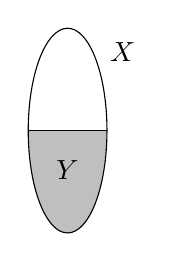
\begin{tikzpicture}
      \fill [gray!50!white] (-0.5, 0) arc (180:360:0.5 and 1.3) -- cycle;
      \draw (0, 0) ellipse (0.5 and 1.3);
      \draw (-0.5, 0) -- (0.5, 0);
      \node at (0, -0.5) {$Y$};
      \node at (0.7, 1) {$X$};
    \end{tikzpicture}
  \end{center}
\end{defi}

\begin{eg}
  For any $x\in X$, the set $I_x = \{y\in x: y < x\}$ is an initial segment. However, not every initial segment of $X$ need to be in this form. For example, $\{x: x\leq 3\}\subseteq \R$ and $\{x: x < 0\text{ or }x^2 < 2\}\subseteq \Q$ are both initial segments not of this form.
\end{eg}

The next nice property of well-orders we have is that every proper initial segment is of this form.
\begin{prop}
  Every initial segment $Y$ of a well-ordered set $X$ is of the form $I_x = \{y\in X: y < x\}$.
\end{prop}

\begin{proof}
  Take $x = \min X\setminus Y$. Then for any $y\in I_x$, we have $y < x$. So $y \in Y$ by definition of $x$. So $I_x \subseteq Y$.

  On the other hand, if $y \in Y$, then definitely $y \not= x$. We also cannot have $y > x$ since this implies $x \in Y$. Hence we must have $y < x$. So $y \in I_x$. Hence $Y \subseteq I_x$. So $Y = I_x$.
\end{proof}

The next nice property we want to show is that in a well-ordering $X$, \emph{every} subset $S$ is isomorphic to an initial segment.

Note that this is \emph{very} false for a general total order. For example, in $\Z$, no initial segment is isomorphic to the subset $\{1, 2, 3\}$ since every initial segment of $\Z$ is either infinite or empty. Alternatively, in $\R$, $\Q$ is not isomorphic to an initial segment.

It is intuitively obvious how we can prove this. We simply send the minimum element of $S$ to the minimum of $X$, and the continue recursively. However, how can we justify recursion? If we have the well-order $\{\frac{1}{2}, \frac{2}{3}, \frac{3}{4}, \cdots, 1\}$, then we will never reach $1$ if we attempt to write down each step of the recursion, since we can only get there after infinitely many steps. We will need to define some sort of ``infinite recursion'' to justify our recursion on general well-orders.

We first define the restriction of a function:
\begin{defi}[Restriction of function]
  For $f: A\to B$ and $C\subseteq A$, the \emph{restriction} of $f$ to $C$ is
  \[
    f|_C = \{(x, f(x)): x\in C\}.
  \]
\end{defi}
In this theorem (and the subsequent proof), we are treating functions as explicitly a set of ordered pairs $(x, f(x))$. We will perform set operations on functions and use unions to ``stitch together'' functions.

\begin{thm}[Definition by recursion]
  Let $X$ be a well-ordered set and $Y$ be any set. Then for any function $G: \P(X\times Y)\to Y$, there exists a function $f:X\to Y$ such that
  \[
    f(x) = G(f|_{I_x})
  \]
  for all $x$.

  This is a rather weird definition. Intuitively, it means that $G$ takes previous values of $f(x)$ and returns the desired output. This means that in defining $f$ at $x$, we are allowed to make use of values of $f$ on $I_x$. For example, we define $f(n) = n f(n - 1)$ for the factorial function, with $f(0) = 1$.
\end{thm}

\begin{proof}
  We might want to jump into the proof and define $f(0) = G(\emptyset)$, where $0$ is the minimum element. Then we define $f(1) = G(f(0))$ etc. But doing so is simply recursion, which is the thing we want to prove that works!

  Instead, we use the following clever trick: We define an ``$h$ is an attempt'' to mean
  \begin{center}
    $h: I \to Y$ for some initial segment $I$ of $X$, and $h(x) = G(h|_{I_x})$ for $x\in I$.
  \end{center}
  The idea is to show that for any $x$, there is an attempt $h$ that is defined at $x$. Then take the value $f(x)$ to be $h(x)$. However, we must show this is well-defined first:

  If attempts $h$ and $h'$ are defined at $x$, then $h(x) = h'(x)$. By induction on $x$, it is enough to show that $h(x) = h'(x)$ assuming $h(y) = h'(y)$ for all $y < x$. But then $h(x) = G(h|_{I_x}) = G(h'|_{I_x}) = h'(x)$. So done.

  Now let's show that for any $x$, there must exist an attempt $h$ that is defined at $x$. Again, we may assume (by induction) that for each $y < x$, there exists an attempt $h_y$ defined at $y$. Then we put all these functions together, and take $h' = \bigcup_{y < x} h_y$. This is defined for all $y < x$, and is well-defined since the $h_y$ never disagree.

  Finally, add to it $(x, G(h'|_{I_x}))$. Then $h = h'\cup (x, G(h'|_{I_x}))$ is an attempt defined at $x$.

  Now define $f:X\to Y$ by $f(x) = y$ if there exists an attempt $h$, defined at $x$, with $h(x) = y$.

  We finally show uniqueness by induction on $x$: suppose $f$ and $f'$ both work. Then if $f(y) = f'(y)$ for all $y < x$, then $f(x) = f'(x)$ by definition. So for all $x$, $f'(x) = f(x)$.
\end{proof}
With the tool of recursion, we can prove that every subset of a well-order.

\begin{prop}[Subset collapse]
  Let $X$ be a well-ordering and let $Y\subseteq X$. Then $Y$ is isomorphic to an initial segment of $X$. Moreover, this initial segment is unique.
\end{prop}

\begin{proof}
  For $f: Y\to X$ to be an order-preserving bijection with an initial segment of $X$, we need to map $x$ to the smallest thing not yet mapped to, ie.
  \[
    f(x) = \min (X\setminus \{f(y): y < x\}).
  \]
  To be able to take the minimum, we have to make sure the set is non-empty, ie. $\{f(y): y < x\} \not= X$. We can show this by proving that $f(z) < x$ for all $z < x$ by induction, and hence $x \not\in \{f(y): y < x\}$.

  Then by the recursion theorem, this function exists and is unique.
\end{proof}
This implies that a well-ordered $X$ can \emph{never} be isomorphic to a proper initial segment of itself. This is since $X$ is isomorphic to itself by the identity function, and uniqueness shows that it cannot be isomorphic to another initial segment.

Using the idea of initial segments, we can define an order comparing different well-orders themselves.
\begin{notation}
  Write $X\leq Y$ if $X$ is isomorphic to an initial segment of $Y$.

  We write $X < Y$ if $X\leq Y$ but $X$ is not isomorphic to $Y$, ie. $X$ is isomorphic to a proper initial segment of $Y$.
\end{notation}

\begin{eg}
  If $X = \N$, $Y = \{\frac{1}{2}, \frac{2}{3}, \frac{3}{4},\cdots\}\cup \{1\}$, then $X \leq Y$.
\end{eg}

We will show that this is a total order. Of course, we identify two well-orders as ``equal'' when they are isomorphic.

Reflexivity and transitivity are straightforward. So we prove trichotomy and antisymmetry:
\begin{thm}
  Let $X, Y$ be well-orderings. Then $X\leq Y$ or $Y \leq X$.
\end{thm}

\begin{proof}
  We attempt to define $f: X\to Y$ by
  \[
    f(x) = \min (Y\setminus \{f(y): y < x\}).
  \]
  By the law of excluded middle, this function is either well-defined or not.

  If it is well-defined, then it is an isomorphism from $X$ to an initial segment of $Y$.

  If it is not, then there is some $x$ such that $\{f(y): y < x\} = Y$ and we cannot take the minimum. Then $f$ is a bijection between $I_x = \{y: y < x\}$ and $Y$. So $f$ is an isomorphism between $Y$ and an initial segment of $X$.

  Hence either $X \leq Y$ or $Y \leq X$.
\end{proof}

\begin{thm}
  Let $X, Y$ be well-orderings with $X\leq Y$ and $Y \leq X$. Then $X$ and $Y$ are isomorphic.
\end{thm}

\begin{proof}
  Since $X \leq Y$, there is an order-preserving function $f: X\to Y$ that bijects $X$ with an initial segment of $Y$. Similarly, since $Y \leq X$, we get an analogous $g: Y\to X$. Then $g\circ f: X\to X$ defines a bijection between $X$ and an initial segment of $X$.

  Since there is no bijection between $X$ and a \emph{proper} initial segment of itself, the image of $g\circ f$ must be $X$ itself. Hence $g\circ f$ is a bijection.

  Similarly, $f\circ g$ is a bijection. Hence $f$ and $g$ are both bijections, and $X$ and $Y$ are isomorphic.
\end{proof}

\subsection{New well-orderings from old}
Given a well-ordering $X$, we want to create more well-orderings. We've previously shown that we can create a shorter one by taking an initial segment. In this section, we will explore two ways to make \emph{longer} well-orderings.

\subsubsection*{Add one element}
We can extend a well-ordering by exactly one element. This is known as the \emph{successor}.
\begin{defi}[Successor]
  Given $X$, choose some $x\not\in X$ and define a well-ordering on $X\cup \{x\}$ by setting $y < x$ for all $y \in X$. This is the \emph{successor} of $X$, written $X^+$.
\end{defi}
We clearly have $X < X^+$.
\subsubsection*{Put some together}
More interestingly, we want to ``stitch together'' many well-orderings. However, we cannot just arbitrarily stitch well-orderings together. The well-orderings must satisfy certain nice conditions for this to be well-defined.

\begin{defi}[Extension]
  For well-orderings $(X, <_X)$ and $(Y, <_Y)$, we say $Y$ \emph{extends} $X$ if $X$ is a proper initial segment of $Y$ and $<_X$ and $<_Y$ agree when defined.
\end{defi}
Note that we explicitly require $X$ to be an initial segment of $Y$. $X$ simply being a \emph{subset} of $Y$ will not work, for reasons that will become clear shortly.

\begin{defi}[Nested family]
  We say well-orderings $\{X_i: i\in I\}$ form a \emph{nested} family if for any $i, j\in I$, either $X_i$ extends $X_j$, or $X_j$ extends $X_i$.
\end{defi}

\begin{prop}
  Let $\{X_i: i\in I\}$ be a nested set of well-orderings. Then there exists a well-ordering $X$ with $X_i\leq X$ for all $i$.
\end{prop}

\begin{proof}
  Let $X = \bigcup_{i\in I}X_i$ with $<$ defined on $X$ as $\bigcup_{i\in I} <_i$ (where $<_i$ is the ordering of $X_i$), ie. we inherit the orders from the $X_i$'s. This is clearly a total ordering. Since $\{X_i: i \in I\}$ is a nested family, each $X_i$ is an initial segment of $X$.

  To show that it is a well-ordering, let $S\subseteq X$ be a non-empty subset of $X$. Then $S\cap X_i$ is non-empty for some $i$. Let $x$ be the minimum element (in $X_i$) of $S\cap X_i$. Then also for any $y\in S$, we must have $x \leq y$, as $X_i$ is an initial segment of $X$.
\end{proof}
Note that if we didn't require $X$ to be an initial segment of $Y$ when defining 'extension', then the above proof will not work. For example, we can take the collection of all subsets $X_n = \{x \geq -n: x\in \Z\}$, and their union would be $\Z$, which is not well-ordered.

\subsection{Ordinals}
We have already shown that the collection of all well-orderings is a total order. But is it a well-ordering itself? To investigate this issue further, we first define ourselves a convenient way of talking about well-orderings.

\begin{defi}[Ordinal]
  An \emph{ordinal} is a well-ordered set, with two regarded as the same if they are isomorphic. We write ordinals as Greek letters $\alpha, \beta$ etc.
\end{defi}
We would want to define ordinals as equivalence classes of well-orders under isomorphism, but we cannot, because they do not form a set. We will provide a formal definition of ordinals later when we study set theory.

\begin{defi}[Order type]
  If a well-ordering $X$ has corresponding ordinal $\alpha$, we say $X$ has \emph{order type} $\alpha$, and write $\otp(X) = \alpha$.
\end{defi}

\begin{notation}
  For each $k\in \N$, we write $k$ for the order type of the (unique) well-ordering of size $k$. We write $\omega$ for the order type of $\N$.
\end{notation}

\begin{eg}
  In $\R$, $\{2, 3, 5 ,6\}$ has order type 4. $\{\frac{1}{2}, \frac{2}{3}, \frac{3}{4}, \cdots\}$ has order type $\omega$.
\end{eg}

\begin{notation}
  For ordinals $\alpha, \beta$, write $\alpha \leq \beta$ if $X\leq Y$ for some $X$ of order type $\alpha$, $Y$ of order type $\beta$. This does not depend on the choice of $X$ and $Y$ (since any two choices must be isomorphic).
\end{notation}

\begin{prop}
  Let $\alpha$ be an ordinal. Then the ordinals $<\alpha$ form a well-ordering of order type $\alpha$.
\end{prop}

\begin{notation}
  Write $I_\alpha = \{\beta: \beta < \alpha\}$.
\end{notation}

\begin{proof}
  Let $X$ have order type $\alpha$. The well-orderings $< X$ are precisely (up to isomorphism) the proper initial segments of $X$ (by uniqueness of subset collapse). But these are the $I_x$ for all $x\in X$. So we can biject $X$ with the well-orderings $< X$ by $x\mapsto I_x$.
\end{proof}

Finally, we can prove that the ordinals are well-ordered.
\begin{prop}
  Let $S$ be a non-empty set of ordinals. Then $S$ has a least element.
\end{prop}

\begin{proof}
  Choose $\alpha\in S$. If it is minimal, done.

  If not, then $S\cap I_\alpha$ is non-empty. But $I_\alpha$ is well-ordered. So $S\cap I_\alpha$ has a least element, $\beta$. Then this is a minimal element of $S$.
\end{proof}

However, it would be wrong to say that the ordinals form a well-ordered \emph{set}, for the very reason that they don't form a set.
\begin{thm}[Burali-Forti paradox]
  The ordinals do not form a set.
\end{thm}

\begin{proof}
  Suppose not. Let $X$ be the set of ordinals. Then $X$ is a well-ordering. Let its order-type be $\alpha$. Then $X$ is isomorphic to $I_\alpha$, a proper initial subset of $X$. Contradiction.
\end{proof}

Recall that we could create new well-orderings from old via adding one element and taking unions. We can translate these into ordinal language.

Given an ordinal $\alpha$, suppose that $X$ is the corresponding well-order. Then we define $\alpha^+$ to be the order type of $X^+$.

If we have a set $\{\alpha_i: i \in I\}$ of ordinals, we can stitch them together to form a new well-order. In particular, we apply ``nested well-orders'' to the initial segments $\{I_{\alpha_i}: i \in I\}$. This produces an upper bound of the ordinals $\alpha_i$. Since the ordinals are well-ordered, we know that there is a \emph{least} upper bound. We call this the \emph{supremum} of the set $\{\alpha_i: i \in I\}$, written $\sup\{\alpha_i: i \in I\}$. In fact, the upper bound created by nesting well-orders is the least upper bound.

\begin{eg}
  $\{2, 4, 6, 8, \cdots\}$ has supremum $\omega$.
\end{eg}

Now we have two ways of producing ordinals: $+1$ and supremum.

We can generate a lot of ordinals now:
\begin{center}
  \begin{tabular}{ccccccc}
    0 & $\omega\cdot 2 + 1$ & $\omega^2 + 1$ & $\omega^2\cdot 3$ & $\omega^{\omega + 2}$ & $\varepsilon_0 + 1$ \\
    1 & $\omega\cdot 2 + 2$ & $\omega^2 + 2$ & $\omega^2\cdot 4$ & $\vdots$ & $\vdots$ \\
    2 & $\omega\cdot 2 + 3$ & $\omega^2 + 3$ & $\omega^2\cdot 5$ & $\omega^{\omega \cdot 2}$ & $\varepsilon_0 \cdot 2$ \\
    $\vdots$ & $\vdots$ & $\vdots$ & $\vdots$ & $\vdots$ & $\vdots$ \\
    $\omega$ & $\omega\cdot 3$ & $\omega^2 + \omega$ & $\omega^3$ & $\omega^{\omega^2}$ & $\varepsilon_0^2$ \\
    $\omega + 1$ & $\omega\cdot 4$ & $\vdots$ & $\vdots$ & $\vdots$ & $\vdots$ \\
    $\omega + 2$ & $\omega\cdot 5$ & $\omega^2 + \omega \cdot 2$ & $\omega^\omega$ & $\omega^{\omega^{\omega}}$ & $\varepsilon_0^{\varepsilon_0}$ \\
    $\vdots$ & $\vdots$ & $\vdots$ & $\vdots$ & $\vdots$ & $\vdots$ \\
    $\omega + \omega = \omega\cdot 2$ & $\omega\cdot \omega = \omega^2$ & $\omega^2 + \omega^2 = \omega^2 \cdot 2$ & $\omega^{\omega + 1}$ & $\omega^{\omega^{.^{.^.}}} = \varepsilon_0$ & $\varepsilon_0^{\varepsilon_0^{.^{.^.}}} = \varepsilon_1$ \\
  \end{tabular}
\end{center}
Here we introduced a lot of different notations. For example, we wrote $\omega + 1$ to mean $\omega^+$, and $\omega\cdot 2 = \sup\{\omega, \omega + 1, \omega + 2, \cdots\}$. We will formally define these notations later.

We have written a lot of ordinals above, some of which are really huge. However, all the ordinals above are countable. The operations we have done so far is adding one element and taking countable unions. So the results are all countable. So is there an uncountable ordinal?

\begin{thm}
  There is an uncountable ordinal.
\end{thm}

\begin{proof}
  This is easy by looking at the supremum of the set of all countable ordinals. However, this works only if the collection of countable ordinals is a set.

  Let $A = \{R\in \P(\N\times \N): R \text{ is a well-ordering of a subset of }\N\}$. So $A \subseteq \P(\N\times \N)$. Then $B = \{\text{order type of }R: R\in A\}$ is the set of all countable ordinals.

  Let $\omega_1 = \sup B$. Then $\omega_1$ is uncountable. Indeed, if $\omega_1$ were countable, then it would be the greatest countable ordinal, but $\omega_1 + 1$ is greater and is also countable.
\end{proof}

By definition, $\omega_1$ is the \emph{least} uncountable ordinal, and everything in our previous big list of ordinals is less than $\omega_1$.

There are two strange properties of $\omega_1$:
\begin{enumerate}
  \item $\omega_1$ is an uncountable ordering, yet for every $x\in \omega_1$, the set $\{y: y< x\}$ is countable.
  \item Every sequence in $\omega_1$ is bounded, since its supremum is a countable union of countable sets, which is countable.
\end{enumerate}

In general, we have the following theorem:
\begin{thm}[Hartogs' lemma]
  For any set $X$, there is an ordinal that does not inject into $X$.
\end{thm}

\begin{proof}
  As before, with $B = \{\alpha: \alpha\text{ injects into }X\}$.
\end{proof}

\begin{notation}
  Write $\gamma(X)$ for the least ordinal that does not inject into $X$. eg. $\gamma(\omega) = \omega_1$.
\end{notation}

\subsection{Successors and limits}
In general, we can divide ordinals into two categories. The criteria is as follows:

Given an ordinal $\alpha$, is there a greatest element of $\alpha$? ie. does $I_\alpha = \{\beta: \beta < \alpha\}$ have a greatest element?

If yes, say $\beta$ is the greatest element. Then $\gamma\in I_\alpha \Leftrightarrow \gamma \leq \beta$. So $I_\alpha = \{\beta\}\cup I_\beta$. In other words, $\alpha = \beta^+$.

\begin{defi}[Successor ordinal]
  An ordinal $\alpha$ is a \emph{successor ordinal} if there is a greatest element $\beta$ below it. Then $\alpha = \beta^+$.
\end{defi}

On the other hand, if no, then for any $\gamma < \alpha$, there exists $\beta < \alpha$ such that $\beta > \gamma$. So $\alpha = \sup \{\beta: \beta < \alpha\}$.
\begin{defi}[Limit ordinal]
  An ordinal $\alpha$ is a limit if it has no greatest element below it. We usually write $\lambda$ for limit ordinals.
\end{defi}

\begin{eg}
  $5$ and $\omega^+$ are successors. $\omega$ and $0$ are limits ($0$ is a limit because it has no element below it, let alone a greatest one!.
\end{eg}

\subsection{Ordinal arithmetic}
We want to define ordinals arithmetic such as $+$ and $\times$, so that we can make formal sense out of our notations such as $\omega + \omega$ in our huge list of ordinals.

We first start with addition.
\begin{defi}[Ordinal addition (inductive)]
  Define $\alpha + \beta$ by recursion on $\beta$ ($\alpha$ is fixed):
  \begin{itemize}
    \item $\alpha + 0 = \alpha$.
    \item $\alpha + \beta^+ = (\alpha + \beta)^+$.
    \item $\alpha + \lambda = \sup \{\alpha + \gamma: \gamma < \lambda\}$ for non-zero limit $\lambda$.
  \end{itemize}
\end{defi}
Note that officially, we cannot do ``recursion on the ordinals'', since the ordinals don't form a set. So what we officially do is that we define $\alpha + \gamma$ on $\{\gamma: \gamma < \beta\}$ recursively for each ordinal $\beta$. Then by uniqueness of recursions, we can show that this addition is well-defined.

\begin{eg}
  $\omega + 1 = (\omega + 0)^+ = \omega^+$.

  $\omega + 2 = (\omega + 1)^+ = \omega^{++}$.

  $1 + \omega = \sup\{ 1 + n: n \leq \omega\} = \sup\{1, 2, 3, \cdots\} = \omega$.
\end{eg}
It is very important to note that addition is not commutative! This asymmetry arises from our decision to perform recursion on $\beta$ instead of $\alpha$.

On the other hand, addition \emph{is} associative.
\begin{prop}
  Addition is associative, ie. $(\alpha + \beta) + \gamma = \alpha + (\beta + \gamma)$.
\end{prop}

\begin{proof}
  Since we define addition by recursion, it makes sense to prove this by induction. Since we recursed on the right-hand term in the definition, it only makes sense to induct on $\gamma$ (and fix $\alpha + \beta$).

\begin{enumerate}
  \item If $\gamma = 0$, then $\alpha + (\beta + 0) = \alpha + \beta = (\alpha + \beta) + 0$.
  \item If $\gamma = \delta^+$ is a successor, then
    \begin{align*}
      \alpha + (\beta + \delta^+) &= \alpha + (\beta + \delta)^+\\
      &= [\alpha + (\beta + \delta)]^+\\
      &= [(\alpha + \beta) + \delta]^+\\
      &= (\alpha + \beta) + \delta^+\\
      &= (\alpha + \beta) + \gamma.
    \end{align*}
  \item If $\gamma$ is a limit ordinal, we have
    \begin{align*}
      (\alpha + \beta) + \lambda &= \sup\{(\alpha + \beta) + \gamma: \gamma < \lambda\}\\
      &= \sup\{\alpha + (\beta + \gamma): \gamma < \lambda\}
    \end{align*}
    If we want to evaluate $\alpha + (\beta + \lambda)$, we have to first know whether $\beta + \lambda$ is a successor or a limit. We now claim it is a limit:

    $\beta + \lambda = \sup\{\beta + \gamma: \gamma < \lambda\}$. We show that this cannot have a greatest element: for any $\beta + \gamma$, since $\lambda$ is a limit ordinal, we can find a $\gamma'$ such that $\gamma < \gamma' < \lambda$. So $\beta + \gamma' > \beta + \gamma$. So $\beta + \gamma$ cannot be the greatest element.

    So
    \[
      \alpha + (\beta + \lambda) = \sup\{\alpha + \delta: \delta < \beta + \lambda\}.
    \]
    We need to show that
    \[
      \sup\{\alpha + \delta: \delta < \beta + \lambda\} = \sup\{\alpha + (\beta + \gamma): \gamma < \lambda\}.
    \]
    Note that the two sets are not equal. For example, if $\beta = 3$ and $\lambda = \omega$, then the left contains $\alpha + 2$ but the right does not.

    So we show that the left is both $\geq$ and $\leq$ the right.

    $\geq$: Each element of the right hand set is an element of the left.

    $\leq$: For $\delta < \beta + \lambda$, we have $\delta < \sup \{\beta + \gamma: \gamma < \lambda\}$. So $\delta < \beta + \gamma$ for some $\gamma < \lambda$. Hence $\alpha + \delta < \alpha + (\beta + \gamma)$.
\end{enumerate}
\end{proof}
Note that it is easy to prove that $\beta < \gamma \Rightarrow \alpha + \beta < \alpha + \gamma$ by induction on $\gamma$ (which we implicitly assumed above). But it is not true if we add on the right: $1 < 2$ but $1 + \omega = 2 + \omega$.

The definition we had above is called the \emph{inductive} definition. There is an alternative definition of $+$ based on actual well-orders. This is known as the \emph{synthetic} definition.

Intuitively, we first write out all the elements of $\alpha$, then write out all the elements of $\beta$ after it. The $\alpha + \beta$ is the order type of the combined mess.

\begin{defi}[Ordinal addition (synthetic)]
  $\alpha + \beta$ is the order type of $\alpha \sqcup \beta$ ($\alpha$ disjoint union $\beta$, eg. $\alpha\times \{0\}\cup \beta\times \{1\}$), with all $\alpha$ before all of $\beta$
  \[
    \alpha + \beta = \underbracket{\quad\quad\vphantom{\beta}\alpha\vphantom{\beta}\quad\quad}\underbracket{\quad\;\beta\;\quad}
  \]
\end{defi}
\begin{eg}
  $\omega + 1 = \omega^+$.

  $1 + \omega = \omega$.
\end{eg}

With this definition, associativity is trivial:.
\[
  \alpha + (\beta + \gamma) = \underbracket{\quad\quad\vphantom{\beta}\alpha\vphantom{\beta}\quad\quad}\underbracket{\quad\;\beta\;\quad}\underbracket{\quad\gamma\quad} = (\alpha + \beta) + \gamma.
\]
Now that we have given two definitions, we must show that they are the same:
\begin{prop}
  The inductive and synthetic definition of $+$ coincide.
\end{prop}

\begin{proof}
  Write $+$ for inductive definition, and $+'$ for synthetic. We want to show that $\alpha + \beta = \alpha +' \beta$. We induct on $\beta$.

  \begin{enumerate}
    \item $\alpha + 0 = \alpha = \alpha +' 0$.
    \item $\alpha + \beta^+ = (\alpha + \beta)^+ = (\alpha +' \beta)^+ = \otp\underbracket{\quad\vphantom\beta\alpha\vphantom\beta\quad}\underbracket{\quad\beta\quad}\underbracket{\vphantom\beta\cdot\vphantom\beta} = \alpha +' \beta^+$
    \item $\alpha + \lambda = \sup\{\alpha + \gamma: \gamma < \lambda\} = \sup \{\alpha +' \gamma: \gamma < \lambda\} = \alpha +' \lambda$. This works because taking the supremum is the same as taking the union.
      \[
        \underbracket{\quad\vphantom\gamma\alpha\vphantom\gamma\quad}\underbracket{\gamma\quad\gamma'\;\gamma''\cdots \lambda}
      \]
  \end{enumerate}
\end{proof}
The synthetic definition is usually easier to work with, if possible. For example, it was very easy to show associativity using the synthetic definition. It is also easier to see why addition is not associative. However, if we want to do induction, the inductive definition is usually easier.

After addition, we can define multiplication. Again, we first give an inductive definition, and then a synthetic one.
\begin{defi}[Ordinal multiplication (inductive)]
  We define $\alpha\cdot \beta$ by induction on $\beta$ by:
  \begin{enumerate}
    \item $\alpha\cdot 0 = 0$.
    \item $\alpha\cdot (\beta^+) = \alpha\cdot \beta + \alpha$.
    \item $\alpha\cdot \lambda = \sup\{\alpha\cdot \gamma: \gamma < \lambda\}$ for $\lambda$ a non-zero limit.
  \end{enumerate}
\end{defi}

\begin{eg}\leavevmode
  \begin{itemize}
    \item $\omega \cdot 1 = \omega\cdot 0 + \omega = 0 + \omega = \omega$.
    \item $\omega \cdot 2 = \omega \cdot 1 + \omega = \omega + \omega$.
    \item $2\cdot \omega = \sup\{2\cdot n: n < \omega\} = \omega$.
    \item $\omega\cdot \omega = \sup \{\omega\cdot n: n < \omega\} = \sup\{\omega, \omega^2, \omega^3, \cdots\}$.
  \end{itemize}
\end{eg}

We also have a synthetic definition.
\begin{defi}[Ordinal multiplication (synthetic)]
  \[
    \beta\left\{
      \begin{array}{c}
        \underbracket{\quad\alpha\quad} \\
        \vdots \\
        \underbracket{\quad\alpha\quad} \\
        \underbracket{\quad\alpha\quad}
      \end{array}\right.
    \]
  Formally, $\alpha\cdot \beta$ is the order type of $\alpha\times \beta$, with $(x, y) < (x', y')$ if $y < y'$ or ($y = y'$ and $x < x'$).
\end{defi}

\begin{eg}
  $\displaystyle\omega\cdot 2 =
  \begin{array}{c}
    \underbracket{\quad\omega\quad}\\
    \underbracket{\quad\omega\quad}
  \end{array} = \omega + \omega$.

  Also $2\cdot \omega = \omega\left\{
  \begin{array}{c}
    \underbracket{\,\cdot\,\cdot\,} \\
    \vdots \\
    \underbracket{\,\cdot\,\cdot\,} \\
    \underbracket{\,\cdot\,\cdot\,} \\
  \end{array}\right. = \omega$
\end{eg}
We can check that the definitions coincide, prove associativity etc. similar to what we did for addition.

We can define ordinal exponentiation, towers etc. similarly:
\begin{defi}[Ordinal exponentiation (inductive)]
  $\alpha^\beta$ is defined as
  \begin{enumerate}
    \item $\alpha^0 = 1$
    \item $\alpha^{\beta^+} = \alpha^\beta \cdot \alpha$
    \item $\alpha^{\lambda} = \sup \{\alpha^\gamma: \gamma< \lambda\}$.
  \end{enumerate}
\end{defi}

\begin{eg}
  $\omega^1 = \omega^0\cdot \omega = 1\cdot \omega = \omega$.

  $\omega^2 = \omega^1\cdot \omega = \omega\cdot \omega$.

  $2^{\omega} = \sup \{2^n: n < \omega\} = \omega$.
\end{eg}

\section{Posets and Zorn's lemma}
\label{sec:poset}
In this chapter, we study \emph{partial orders}. While there are many examples of partial orders, the most important example is the power set $\P(X)$ for any set $X$, ordered under inclusion. We will also consider subsets of the power set.

The two main theorems of this chapter are Knaster-Tarski fixed point theorem and Zorn's lemma. We will use Zorn's lemma to prove a lot of useful results in different fields, including the completeness theorem in propositional calculus. Finally, we will investigate the relationship between Zorn's lemma and Axiom of Choice.

\subsection{Partial orders}
\begin{defi}[Partial ordering (poset)]
  A \emph{partially ordered set} or \emph{poset} is a pair $(X, \leq)$, where $X$ is a set and $\leq$ is a relation on $X$ that satisfies
  \begin{enumerate}
    \item $x\leq x$ for all $x\in X$ \hfill (reflexivity)
    \item $x \leq y$ and $y \leq z \Rightarrow x \leq z$ \hfill (transitivity)
    \item $x \leq y$ and $y \leq x \Rightarrow x = y$ \hfill (antisymmetry)
  \end{enumerate}
  We write $x < y$ to mean $ x\leq y$ and $x\not= y$. We can also define posets in terms of~$<$:
  \begin{enumerate}
    \item $x \not< x$ for all $x\in X$ \hfill (irreflexive)
    \item $x < y$ and $y < z\Rightarrow x < z$ \hfill (transitive)
  \end{enumerate}
\end{defi}

\begin{eg}\leavevmode
  \begin{enumerate}
    \item Any total order is (trivially) a partial order.
    \item $\N$ with ``$x\leq y$'' if $x \mid y$ is a partial order.
    \item $\P(S)$ with $\subseteq$ for any set $S$ is a partial order.
    \item Any subset of $\P(S)$ with inclusion is a partial order.
    \item We can use a diagram
      \begin{center}
        \begin{tikzpicture}[grow=up]
          \node {a}
          child {
            node {b} edge from parent
            child {
              node {c} edge from parent
            }
          }
          child {
            node {d} edge from parent
            child {
              node {e} edge from parent
            }
          };
        \end{tikzpicture}
      \end{center}
      Where ``above'' means ``greater''. So $a \leq b\leq c$, $a \leq d\leq e$, and what follows by transitivity. This is a Hasse diagram.

      \begin{defi}[Hasse diagram]
        A \emph{Hasse diagram} for a poset $X$ consists of a drawing of the points of $X$ in the plane with an upwards line from $x$ to $y$ if $y$ \emph{covers} $x$:
      \end{defi}
      \begin{defi}[Cover]
        In a poset, $y$ \emph{covers} $x$ if $y > x$ and no $z$ has $y > z > x$.
      \end{defi}
      Hasse diagrams can be useful --- eg. $\N$, or useless, eg. $\Q$.
    \item The following example shows that we cannot assign ``heights'' or ``ranks'' to posets:
      \begin{center}
        \begin{tikzpicture}
          \node (a) {$a$};
          \node[above=0.5 of a] (dummy1) {};
          \node[above=0.5 of dummy1] (dummy2) {};
          \node[above=0.5 of dummy2] (dummy3) {};

          \node[right=of dummy1] (d) {$d$} edge (a);
          \node[left=of dummy2] (b) {$b$} edge (a);
          \node[right=of dummy3] (e) {$e$} edge (d);
          \node [above=0.5 of dummy3] {$c$} edge (b) edge (e);
        \end{tikzpicture}
      \end{center}
    \item We can also have complicated structures:
      \begin{center}
        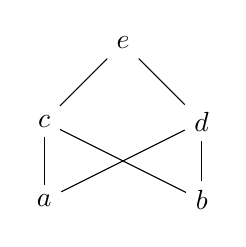
\begin{tikzpicture}[node distance=1]
          \node at (-1, 0) (a) {$a$};
          \node at (1, 0) (b) {$b$};
          \node at (-1, 1) (c) {$c$} edge (a) edge (b);
          \node at (1, 1) (d) {$d$} edge (a) edge (b);
          \node at (0, 2) {$e$} edge (c) edge (d);
        \end{tikzpicture}
      \end{center}
    \item Or the empty poset (let $X$ be any set and nothing is less than anything else).
  \end{enumerate}
\end{eg}
While there are many examples of posets, all we care about are actually power sets and their subsets only.

Often, we want to study subsets of posets. For example, we might want to know if a subset has a least element. All subsets are equal, but some subsets are more equal than others. A particular interesting class of subsets is a \emph{chain}.
\begin{defi}[Chain and antichain]
  In a poset, a subset $S$ is a \emph{chain} if it is totally ordered, ie. for all $x$, $y$, $x\leq y$ or $y\leq x$. An \emph{antichain} is a subset in which no two things are related.
\end{defi}

\begin{eg}
  In $(\N, \mid )$, $1, 2, 4, 8, 16, \cdots$ is a chain.

  In (v), $\{a, b, c\}$ or $\{a, c\}$ are chains.

  $\R$ is a chain in $\R$.
\end{eg}

\begin{defi}[Upper bound and supremum]
  For $S\subset X$, an \emph{upper bound} for $S$ is an $x\in X$ such that $\forall y\in S: x \geq y$.

  $x\in X$ is a \emph{least upper bound}, \emph{supremum} or \emph{join} of $S$, written $x = \sup S$ or $x = \bigvee S$, if $x$ is an upper bound for $S$, and for all $y \in X$, if $y$ is an upper bound, then $y \geq x$.
\end{defi}

\begin{eg}\leavevmode
  \begin{enumerate}
    \item In $\R$, $\{x: x < \sqrt{2}\}$ has an upper bound $7$, and has a supremum $\sqrt{2}$.

    \item In (v) above, consider $\{a, b\}$. Upper bounds are $b$ and $c$. So $\sup = b$. However, $\{b, d\}$ has no upper bound!
    \item In (vii), $\{a, b\}$ has upper bounds $c, d, e$, but has no \emph{least} upper bound.
  \end{enumerate}
\end{eg}

\begin{defi}[Complete poset]
  A poset $X$ is \emph{complete} if every $S\subseteq X$ has a supremum. In particular, it has a greatest element (ie. $x$ such that $\forall y: x \geq y$), namely $\sup X$, and least element (ie. $x$ such that $\forall y: x \leq y$), namely $\sup \emptyset$.
\end{defi}
It is very important to remember that this definition does \emph{not} require that the subset $S$ is bounded above or non-empty. This is different from the definition of metric space completeness.

\begin{eg}\leavevmode
  \begin{itemize}
    \item $\R$ is not complete because $\R$ itself has no supremum.
    \item $[0, 1]$ is complete because every subset is bounded above, and so has a least upper bound. Also, $\emptyset$ has a supremum of $0$.
    \item $(0, 1)$ is not complete because $(0, 1)$ has no upper bound.
    \item $\P(S)$ for any $S$ is \emph{always} complete, because given any $\{A_i: i\in A\}$, where each $A_i\subseteq S$, $\bigcup A_i$ is its supremum.
  \end{itemize}
\end{eg}

Now we are going to derive fixed-point theorems for complete posets. We start with a few definitions:

\begin{defi}[Fixed point]
  A \emph{fixed point} of a function $f:X\to X$ is an $x$ such that $f(x) = x$.
\end{defi}

\begin{defi}[Order-preserving function]
  For a poset $X$, $f: X\to X$ is \emph{order-preserving} of $x \leq y \Rightarrow f(x) \leq f(y)$.
\end{defi}

\begin{eg}\leavevmode
  \begin{itemize}
    \item On $\N$, $x\mapsto x + 1$ is order-preserving
    \item On $\Z$, $x\mapsto x - 1$ is order-preserving
    \item On $(0, 1)$, $x\mapsto \frac{1 + x}{2}$ is order-preserving (this function halves the distance from $x$ to $1$).
    \item On $\P(S)$, let some fixed $i\in S$. Then $A\mapsto A\cup \{i\}$ is order-preserving.
  \end{itemize}
\end{eg}
Not every order-preserving $f$ has a fixed point (eg. first two above). However, we have
\begin{thm}[Knaster-Tarski fixed point theorem]
  Let $X$ be a complete poset, and $f: X\to X$ be a order-preserving function. Then $f$ has a fixed point.
\end{thm}

\begin{proof}
  To show that $f(x) = x$, we need $f(x) \leq x$ and $f(x) \geq x$. Let's not be too greedy and just want half of it:

  Let $E = \{x: x \leq f(x)\}$. Let $s = \sup E$. We claim that this is a fixed point, by showing $f(s) \leq s$ and $s \leq f(s)$.

  To show $s \leq f(s)$, we use the fact that $s$ is the least upper bound. So if we can show that $f(s)$ is also an upper bound, then $s \leq f(s)$. Now let $x \in E$. So $x\leq s$. Therefore $f(x) \leq f(s)$ by order-preservingness. Since $x \leq f(x)$ (by definition of $E$) $x \leq f(x) \leq f(s)$. So $f(s)$ is an upper bound.

  To show $f(s) \leq s$, we simply have to show $f(s) \in E$, since $s$ is an upper bound. But we already know $s \leq f(s)$. By order-preservingness, $f(s) \leq f(f(s))$. So $f(s)\in E$ by definition.
\end{proof}
While this proof looks rather straightforward, we need to first establish that $s \leq f(s)$, then use this fact to show $f(s) \leq s$. If we decided to show $f(s) \leq s$ first, then we would fail!

The very typical application of Knaster-Tarski is the quick, magic proof of Cantor-Shr\"oder-Bernstein theorem.
\begin{cor}[Cantor-Schr\"oder-Bernstein theorem]
  Let $A, B$ be sets. Let $f: A\to B$ and $g: B\to A$ be injections. Then there is a bijection $h: A\to B$.
\end{cor}

\begin{proof}
  We try to partition $A$ into $P$ and $Q$, and $B$ into $R$ and $S$, such that $f(P) = R$ and $g(S) = Q$. Then we let $h = f$ on $R$ and $g^{-1}$ on $Q$.
  \begin{center}
    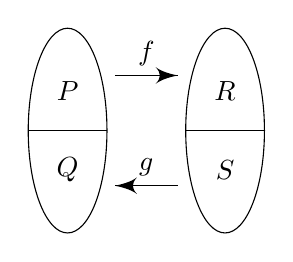
\begin{tikzpicture}
      \draw (-1, 0) ellipse (0.5 and 1.3);
      \draw (-1.5, 0) -- (-0.5, 0);
      \node at (-1, -0.5) {$Q$};
      \node at (-1, 0.5) {$P$};
      \draw (1, 0) ellipse (0.5 and 1.3);
      \draw (0.5, 0) -- (1.5, 0);
      \node at (1, -0.5) {$S$};
      \node at (1, 0.5) {$R$};
      \draw [->] (-0.4, 0.7) -- (0.4, 0.7) node [pos = 0.5, above] {$f$};
      \draw [->] (0.4, -0.7) -- (-0.4, -0.7) node [pos = 0.5, above] {$g$};
    \end{tikzpicture}
  \end{center}
  Since $S = B\setminus R$ and $Q = A \setminus P$, so we want
  \[
    P = A\setminus g(B\setminus f(P))
  \]
  Since the function $P \mapsto A\setminus g(B\setminus f(P))$ from $\P(A)$ to $\P(A)$ is order-preserving (and $\P(a)$ is complete), the result follows.
\end{proof}

The next result we have is Zorn's lemma. The main focus of Zorn's lemma is on \emph{maximal elements}.
\begin{defi}[Maximal element]
  In a poset $X$, $x\in X$ is maximal if no $y\in X$ has $y > x$.
\end{defi}
Caution! Under no circumstances confuse a maximal element with a maximum element, except under confusing circumstances! A maximum element is defined as an $x$ such that all $y\in X$ satisfies $y \leq x$. These two notions are the same in totally ordered sets, but are very different in posets.

\begin{eg}
  In the poset
  \begin{center}
    \begin{tikzpicture}[grow=up]
      \node {a}
      child {
        node {b} edge from parent
        child {
          node {c} edge from parent
        }
      }
      child {
        node {d} edge from parent
        child {
          node {e} edge from parent
        }
      };
    \end{tikzpicture}
  \end{center}
  $c$ and $e$ are maximal.
\end{eg}

Not every poset has a maximal element, eg. $\N, \Q, \R$. In each of these, not only are they incomplete. They have chains that are not bounded above.

\begin{thm}[Zorn's lemma]
  Assuming Axiom of Choice, let $X$ be a (non-empty) poset in which every chain has an upper bound. Then it has a maximal element.
\end{thm}
Note that ``non-empty'' is not a strictly necessary condition, because if $X$ is an empty poset, then the empty chain has no upper bound. So the conditions can never be satisfied.

The actual proof of Zorn's lemma is rather simple, given what we've had so far. We ``hunt'' for the maximal element. We start with $x_0$. If it is maximal, done. If not, we find a bigger $x_1$. If $x_1$ is maximal, done. Otherwise, keep go on.

If we never meet a maximal element, then we have an infinite chain. This has an upper bound $x_\omega$. If this is maximal, done. If not, find $x_{\omega + 1} > x_\omega$. Keep going on.

We have not yet reached a contradiction. But suppose we never meet a maximal element. If $X$ is countable, and we can reach $x_{\omega_1}$, then we have found uncountably many elements in a countable set, which is clearly nonsense!

Since the ordinals can be arbitrarily large (Hartog's lemma), if we never reach a maximal element, then we can get find more elements that $X$ has.

\begin{proof}
  Suppose not. So for each $x\in x$, we have $x'\in X$ with $x' > x$. We denote the-element-larger-than-$x$ by $x'$.

  We know that each chain $C$ has an upper bound, say $u(C)$.

  Let $\gamma = \gamma(X)$, the ordinal-larger-than-$X$ by Hartog's lemma.

  We pick $x\in X$, and define $x_\alpha$ for $\alpha < \gamma$ recursively by
  \begin{itemize}
    \item $x_0 = x$
    \item $x_{\alpha^+} = x_\alpha'$
    \item $x_{\lambda} = u(\{x_\alpha: \alpha < \lambda\})'$ for non-zero limit $\lambda$
  \end{itemize}
  Of course, we have to show that $\{x_\alpha: \alpha < \lambda\}$ is a chain. This is trivial by induction.

  Then $\alpha \mapsto x_\alpha$ is an injection from $\gamma\to X$. Contradiction.
\end{proof}
Note that we could as well have defined $x_\lambda = u(\{x_\alpha : \alpha < \lambda\})$, and we can easily prove it is still an injection. However, we are lazy and put the ``prime'' just to save a few lines of proof.

This proof was rather easy. However, this is only because we are given ordinals, definition by recursion, and Hartog's lemma. Without these tools, it is rather difficult to prove Zorn's lemma.

A typical application of Zorn's lemma is: Does every vector space have a basis? Recall that a \emph{basis} of $V$ is a subset of $V$ that is linearly independent (no finite linear combination $= 0$) and spanning (ie every $x\in V$ is a finite linear combination from it).

\begin{eg}\leavevmode
  \begin{itemize}
    \item Let $V$ be the space of all real polynomials. A basis is $\{1, x, x^2, x^3, \cdots\}$.
    \item Let $V$ be the space of all real sequences. Let $\mathbf{e}_i$ be the sequence with all $0$ except $1$ in the $i$th place. However, $\{\mathbf{e}_i\}$ is not a basis, since $1, 1, \cdots$ cannot be written as a finite linear combination of them. In fact, there is no countable basis (easy exercise). It turns out that there is no ``explicit'' basis.
    \item Take $\R$ as a vector space over $\Q$. A basis here, if exists, is called a Hamel basis.
  \end{itemize}
\end{eg}

Using Zorn's lemma, we can prove that the answer is positive.
\begin{thm}
  Every vector space $V$ has a basis.
\end{thm}

\begin{proof}
  We go for a maximal linearly independent subset.

  Let $X$ be the set of all linearly independent subsets of $V$, ordered by inclusion. We want to find a maximal $B\in X$. Then $B$ is a basis. Otherwise, if $B$ does not span $V$, choose $x\not\in \spn B$. Then $B\cup \{x\}$ is independent, contradicting maximality.

  So we have to find such a maximal $B$. By Zorn's lemma, we simply have to show that every chain has an upper bound.

  Given a chain $\{A_i: i\in I\}$ in $X$, a reasonable guess is to try the union. Let $A = \bigcup A_i$. Then $A\subseteq A_i$ for all $i$, by definition. So it is enough to check that $A\in X$, ie. is linearly independent.

  Suppose not. Say $\lambda_1x_1 + \cdots + \lambda_nx_n = 0$ for some $\lambda_1 \cdots \lambda_n$ scalars (not all $0$). Suppose $x_1 \in A_{i_1}, \cdots x_n \in A_{i_n}$ for some $i_1, \cdots i_n \in I$. Then there is some $A_{i_m}$ that contains all $A_{i_k}$, since they form a finite chain. So $A_{i_m}$ contains all $x_i$. This contradicts the independence of $A_{i_m}$.

  Hence by Zorn's lemma, $X$ has a maximal element. Done.
\end{proof}

Another application is the completeness theorem for propositional logic when $P$, the primitives, can be uncountable.

\begin{thm}[Model existence theorem (uncountable case)]
  Let $S\subseteq L(P)$ for any set of primitive propositions $P$. Then if $S$ is consistent, $S$ has a model.
\end{thm}

\begin{proof}
  We need a consistent $\bar S \subseteq S$ such that $\forall t\in L$, $t\in \bar S$ or $\neg t\in \bar S$. Then we have a valuation $v(t) = \begin{cases} 1 & t\in \bar S \\ 0 & t\not\in \bar S\end{cases}$, as in our original proof for the countable case.

  So we seek a \emph{maximal} consistent $\bar S\supseteq S$. If $\bar S$ is maximal, then if $t\not\in \bar S$, then we must have $\bar S \cup \{t\}$ inconsistent, ie. $\bar S \cup \{t\}\vdash \bot$. By deduction theorem, this means that $\bar S \vdash \neg t$. By maximality, we must have $\neg t \in \bar S$. So either $t$ or $\neg t$ is in $\bar S$.

  Now we show that there is such a maximal $\bar S$. Let $X = \{ T\subseteq L: T\text{ is consistent }, T\supseteq S\}$. Then $X\not=\emptyset$ since $S\in X$. We show that any non-empty chain has an upper bound. An obvious choice is, again the union.

  Let $\{T_i: i\in I\}$ be a non-empty chain. Let $T = \bigcup T_i$. Then $T\supseteq T_i$ for all $i$. So to show that $T$ is an upper bound, we have to show $T\in X$.

  Certainly, $T\supseteq S$, as any $T_i$ contains $S$ (and the chain is non-empty). So we want to show $T$ is consistent. Suppose $T\vdash \bot$. So we have $t_1, \cdots, t_n \in T$ with $\{t_1, \cdots, t_n\} \vdash \bot$, since proofs are finite. Then some $T_k$ contains all $t_i$ since $T_i$ are nested. So $T_k$ is inconsistent. This is a contradiction. Therefore $T$ must be consistent.

  Hence by Zorn's lemma, there is a maximal element of $X$.
\end{proof}
This proof is basically the same proof that every vector space has a basis! In fact, most proofs involving Zorn's lemma are similar.

\subsection{Zorn's lemma and axiom of choice}
Recall that in the proof of Zorn's, we picked $x$, then picked $x'$, then picked $x''$, \emph{ad infinitum}. Here we are making arbitrary choices of $x'$. In particular, we have made infinitely many arbitrary choices.

We did the same in IA Numbers and Sets, when proving a countable union of countable sets is countable, because we chose, for each $A_n$, a listing of $A_n$, and then count them diagonally. We needed to make a choice because each $A_n$ has a lot of possible listings, and we have to pick exactly one.

In terms of ``rules for producing sets'', we are appealing to the axiom of choice, which states that you can pick an element of each $A_i$ whenever $\{A_i: i\in I\}$ is a family of non-empty sets. Formally,
\begin{axiom}[Axiom of choice]
  Given any family $\{A_i: i\in I\}$ of non-empty sets, there is a \emph{choice function} $f: i \to \bigcup A_i$ such that $f(i)\in A_i$.
\end{axiom}
This is of a different character from the other set-building rules (eg. unions and power sets exist). The difference is that the other rules are concrete. We know exactly what $A\cup B$ is, and there is only one possible candidate for what $A\cup B$ might be. ``Union'' uniquely specifies what it produces. However, the choice function is not. $\{A_i:i\in I\}$ can have many choice functions, and the axiom of choice does not give us a solid, explicit choice function. We say the axiom of choice is \emph{non-constructive}.

We are not saying that it's wrong, but it's \emph{weird}. For this reason, it is often of interest to ask ``Did I use AC?'' and ``Do I need AC?''.

(It is important to note that the Axiom of Choice is needed only to make \emph{infinite} choices. It is trivially true if $|I| = 1$, since $A\not=\emptyset$ by definition means $\exists x\in A$. We can also do it for two sets. Similarly, for $|I|$ finite, we can do it by induction. However, in general, AC is required to make infinite choices, ie. it cannot be deduced from the other axioms of set theory)

In the proof of Zorn's we used Choice. However, do we \emph{need} it? Is it possible to prove it without Choice?

The answer is it is necessary, since we can deduce AC from Zorn's. In other words, we can write down a proof of AC from Zorn's, using only the other set-building rules.

\begin{thm}
  Zorn's Lemma $\Leftrightarrow$ Axiom of choice.
\end{thm}

As in the past uses of Zorn's lemma, we have a big scary choice function to produce. We know that we can do it for small cases, such as when $|I| = 1$. So we start with small attempts and show that the maximal attempt is what we want.
\begin{proof}
  We have already proved that AC $\Rightarrow $ Zorn. We now proved the other way round.

  Given a family $\{A_i: i\in I\}$ of non-empty sets. We say a \emph{partial choice function} is a function $f: J\to \bigcup_{i\in I}A_i$ (for some $J\subseteq I$) such that $f(j)\in A$ for all $j\in J$.

  Let $X = \{(J, f): f\text{ is a partial choice function with domain }J\}$. We order by extension, ie. $(J, f) \leq (J', f')$ iff $J\subseteq J'$ and $f'$ agrees with $f$ when both are defined.

  Given a chain $\{(J_k, f_k): k\in K\}$, we have an upper bound $\left(\bigcup J_k, \bigcup f_k\right)$, ie the function obtained by combining all functions in the chain. So by Zorn's, it has a maximal element $(J, f)$.

  Suppose $J \not = I$. Then pick $i\in I\setminus J$. Then pick $x\in A_i$. Set $J' = J\cup \{i\}$ and $f' = f\cup\{(i, x)\}$. Then this is greater than $(J, f)$. This contradicts the maximality of $(J, f)$. So we must have $J = I$, ie. $f$ is a full choice function.
\end{proof}

We have shown that Zorn's lemma is equivalent to the Axiom of Choice. There is a \emph{third} statement that is also equivalent to both of these:
\begin{thm}[Well-ordering theorem]
  Axiom of choice $\Rightarrow$ every set $X$ can be well-ordered.
\end{thm}
This might be very surprising at first for, say $X = \R$, since there is no obvious way we can well-order $\R$. However, it is much less surprising given Hartog's lemma, since Hartog's lemma says that there is a (well-ordered) ordinal even bigger than $\R$. So well-ordering $\R$ shouldn't be hard.

\begin{proof}
  The idea is to pick an element from $X$ and call it the first; pick another element and call it the second, and continue transfinitely until we pick everything.

  For each $A\subseteq X$ with $A\not= X$, we let $y_A$ be an element of $X\setminus A$. Here we are using Choice to pick out $y_A$.

  Define $x_\alpha$ recursively: Having defined $x_{\beta}$ for all $\beta < \alpha$, if $\{x_\beta: \beta < \alpha\} = X$, then stop. Otherwise, set $x_\alpha = y_{\{x_\beta: \beta< \alpha\}}$, ie pick $x_\alpha$ to be something not yet chosen.

  We must stop at some time. Otherwise, we have injected $\gamma(X)$ (ie the ordinal larger than $X$) into $X$, which is a contradiction. So when stop, we have bijected $X$ with an well-ordered set (ie. $I_\alpha$, where $\alpha$ is when you've stopped). Hence we have well-ordered $X$.
\end{proof}

Did we need AC? Yes, trivially.
\begin{thm}
  Well-ordering theorem $\Rightarrow $ Axiom of Choice.
\end{thm}

\begin{proof}
  Given non-empty sets $\{A_i: i\in I\}$, well-order $\bigcup A_i$. Then define $f(i)$ to be the least element of $A_i$.
\end{proof}
Our conclusion is:
\begin{center}
  Axiom of Choice $\Leftrightarrow$ Zorn's lemma $\Leftrightarrow$ Well-ordering theorem.
\end{center}
Before we end, we need to do a small sanity check: we showed that these three statements are equivalents using a lot of ordinal theory. Our proofs above make sense only if we did not use AC when building our ordinal theory. Fortunately, we did not, apart from the remark that $\omega_1$ is not a countable supremum --- which used the fact that a countable union of countable sets is countable.

\subsection{Bourbaki-Witt theorem*}
Finally, we'll quickly present a second (non-examinable) fixed-point theorem. This time, we are concerned about \emph{chain-complete} posets and \emph{inflationary} functions.

\begin{defi}[Chain-complete poset]
  We say a poset $X$ is \emph{chain-complete} if $X \not=\emptyset$ and every non-empty chain has a supremum.
\end{defi}

\begin{eg}\leavevmode
  \begin{itemize}
    \item Every complete poset is chain-complete.
    \item Any finite (non-empty) poset is chain complete, since every chain is finite and has a greatest element.
    \item $\{A\subseteq V: A\text{ is linearly independent}\}$ for any vector space $V$ is chain-complete, as shown in the proof that every vector space has a basis.
  \end{itemize}
\end{eg}

\begin{defi}[Inflationary function]
  A function $f: X\to X$ is \emph{inflationary} if $f(x) \geq x$ for all $x$.
\end{defi}

\begin{thm}[Bourbaki-Witt theorem]
  If $X$ is chain-complete and $f: X\to X$ is inflationary, then $f$ has a fixed point.
\end{thm}
This is follows instantly from Zorn's, since $X$ has a maximal element $x$, and since $f(x) \geq x$, we must have $f(x) = x$. However, we can prove Bourbaki-Witt without choice. In the proof of Zorn's, we had to ``pick'' and $x_1 > x_0$. Here, we can simply let
\[
  x_0 \xmapsto{\,f\,} x_1 \xmapsto{\,f\,} x_2 \xmapsto{\,f\,} x_3 \cdots
\]
Since each chain has a \emph{supremum} instead of an upper bound, we also don't need Choice to pick our favorite upper bound of each chain.

Then we can do the same proof as Zorn's to find a fixed point.

We can view this as the ``AC-free'' part of Zorn's. It can be used to prove Zorn's lemma, but the proof is totally magic.

\section{Predicate logic}
\label{sec:predicate}
In the first chapter, we studied propositional logic. However, it isn't sufficient for most mathematics we do.

In, say, group theory, we have a set of objects, operations and constants. For example, in group theory, we have the operations multiplication $m: A^2 \to A$, inverse $i: A\to A$, and a constant $e\in A$. For each of these, we assign a number known as the \emph{arity}, which specifies how many inputs each operation takes. For example, multiplication has arity 2, inverse has arity 1 and $e$ has arity $0$ (we can view $e$ as a function $A^0 \to A$, that takes no inputs and gives a single output).

The study of these objects is known as \emph{predicate logic}. Compared to propositional logic, we have a much richer language, which includes all the operations and possibly relations. For example, with group theory, we have $m, i, e$ in our language, as well as things like $\forall$, $\Rightarrow$ etc. Note that unlike propositional logic, different theories give rise to different languages.

Instead of a valuation, now we have a \emph{structure}, which is a solid object plus the operations and relations required. For example, a structure of group theory will be an actual concrete group with the group operations.

Similar to what we did in propositional logic, we will take $S\models t$ to mean ``for any structure in which $S$ is true, $t$ is true''. For example, ``Axioms of group theory'' $\models m(e, e) = e$, ie. in any set that satisfies the group axioms, $m(e, e) = e$. We also have $S\vdash t$ meaning we can prove $t$ from $S$.

\subsection{Language of predicate logic}
We start with the definition of the language. This is substantially more complicated than what we've got in propositional logic.
\begin{defi}[Language]
  Let $\Omega$ (function symbols) and $\Pi$ (relation symbols) be disjoint sets, and $\alpha : \Omega\cup\Pi \to \N$ a function ('arity').

  The \emph{language} $L = L(\Omega, \Pi, \alpha)$ is the set of formulae, defined as follows:

  \begin{itemize}
    \item \emph{Variables}: we have some variables $x_1, x_2, \cdots, $ (sometimes we write $x, y, z, \cdots$)
    \item \emph{Terms}: these are defined inductively by
      \begin{enumerate}
        \item Every variable is a term
        \item If $f\in \Omega$, $\alpha(f) = n$, and $t_1, \cdots, t_n$ are terms, then $ft_1\cdots t_n$ is a term. We often write $f(t_1, \cdots, t_n)$ instead.
      \end{enumerate}
      \begin{eg}
        In the language of groups $\Omega = \{m, i, e\}$, $\Pi = \emptyset$, and $\alpha (m) = 2, \alpha(i) = 1, \alpha(e) = 0$. Then $e, x_1, m(x_1, x_2), i(m(x_1, x_1))$ are terms.
      \end{eg}
    \item \emph{Atomic formulae}: there are three sorts:
      \begin{enumerate}
        \item $\bot$
        \item $(s = t)$ for any terms $s, t$.
        \item $(\phi t_1 \cdots t_n)$ for any $\phi\in \Pi$ with $\alpha(\phi) = n$ and $t_1, \cdots, t_n$ terms.
      \end{enumerate}
      \begin{eg}
        In the language of posets, $\Omega = \emptyset$, $\Pi=\{\leq\}$ and $\alpha(\leq) = 2$. Then $(x_1 = x_1)$, $x_1\leq x_2$ (really means $(\leq x_1x_2)$) are atomic formulae.
      \end{eg}
    \item \emph{Formulae}: defined inductively by
      \begin{enumerate}
        \item Atomic formulae are formulae
        \item $(p \Rightarrow q)$ is a formula for any formulae $p, q$.
        \item $(\forall x) p$ is a formula for any formula $p$ and variable $x$.
      \end{enumerate}
      \begin{eg}
        In the language of groups, $e = e$, $x_1 = e$, $m(e, e) = e$, $(\forall x) m(x, i(x)) = e$, $(\forall x)(m(x, x) = e \Rightarrow (\exists y) (m(y, y) = x))$ are formulae.
      \end{eg}
  \end{itemize}
\end{defi}
It is important to note that a formula is a string of meaningless symbol. It doesn't make sense to ask whether it is true or false. In particular, the function and relation symbols are not assigned any meaning. The only thing the language cares is the arity of the symbol.

Again, we have the usual abbreviations $\neg p$, $p\wedge q$, $p\vee q$ etc. Also, we have $(\exists x)p$ for $\neg(\forall x)(\neg p)$.

\begin{defi}[Closed term]
  A term is \emph{closed} if it has no variables.
\end{defi}

\begin{eg}
  In the language of groups, $e, m(e, e)$ are closed terms. However, $m(x, i(x))$ is not closed even though we think it is always $e$. Apart from the fact that it is by definition not closed (has variable $x$), we do not have the groups axioms stating that $m(x, i(x)) = e$.
\end{eg}

\begin{defi}[Free and bound variables]
  An occurrence of a variable $x$ in a formula $p$ is \emph{bound} if it is inside brackets of a $(\forall x)$ quantifier. It is \emph{free} otherwise.
\end{defi}

\begin{eg}
  In $(\forall x)(m(x, x) = e)$, $x$ is a bound variable.

  In $(\forall y)(m(y, y) = x \Rightarrow m(x, y) = m(y, x))$, $y$ is bound while $x$ is free.

  We are technically allowed to have a formula with $x$ both bound and free, but \emph{DO NOT DO IT}. For example, $m(x, x) = e \Rightarrow (\forall x)(\forall y)(m(x, y) = m(y, x))$ is a valid formula (first two $x$ are free, while the others are bound).
\end{eg}

\begin{defi}[Sentence]
  A \emph{sentence} is a formula with no free variables.
\end{defi}

\begin{eg}
  $m(e, e) = e$ and $(\forall x)(m(x, x) = e)$ are sentences, while $m(x, i(x)) = e$ is not.
\end{eg}

\begin{defi}[Substitution]
  For a formula $p$, a variable $x$ and a term $t$, the \emph{substitution} $p[t/x]$ is obtained by replacing each free occurrence of $x$ with $t$.
\end{defi}

\begin{eg}
  If $p$ is the statement $(\exists y)(m(y, y) = x)$, then $p[e/x]$ is $(\exists y)(m(y, y) = e$.
\end{eg}
\subsection{Semantic entailment}
In propositional logic, we can't say whether a proposition is true or false unless we have a valuation. What would be a ``valuation'' in the case of predicate logic? It is a set with the operations of the right arity. We call this a structure.

For example, in the language of groups, a structure is a set $G$ with the correct operations. Note that it does not have to satisfy the group axioms in order to qualify as a structure.

\begin{defi}[Structure]
  An $L$-\emph{structure} is a non-empty set $A$ with a function $f_A: A^n \to A$ for each $f\in \Omega, \alpha(f) = n$, and a relation $\phi_A\subseteq A^n$, for each $\phi\in \Pi$, $\alpha(\phi) = n$.
\end{defi}
Note that we explicitly forbid $A$ from being empty. It is possible to formulate predicate logic that allows empty structures, but we will have to make many weird-looking exceptions when defining our logic system. Since empty structures are mostly uninteresting (and don't exist if there is at least one constant), it isn't a huge problem if we ignore it.

\begin{eg}
  In the language of posets $A$, a structure is a set $A$ with a relation $\leq_A \subseteq A\times A$.

  In the language of groups, a structure is a set $A$ with functions $m_A: A\times A\to A$, $i_A: A\to A$ and $e_A\in A$.
\end{eg}
Again, these need not be genuine posets/groups since we do not have the axioms yet.

Now we want to define ``$p$ holds in $A$'' for a sentence $p\in L$ and a $L$-structure $A$.

For example, we want $(\forall x)(m(x, x) = e)$ to be true in $A$ iff for each $a\in A$, we have $m_A(a, a) = e_A$. So to translate $p$ into something about $A$, you ``add subscript $_A$ to each function-symbol and relation-symbol, insert $\in A$ after the quantifiers, and say it aloud''. We call this the interpretation of the sentence $p$.

This is not great as a definition. So we define it formally, and then quickly forget about it.

\begin{defi}[Interpretation]
  To define the \emph{interpretation} $p_A\in {0, 1}$ for each sentence $p$ and $L$-structure $A$, we define inductively:
  \begin{enumerate}
    \item Closed terms: define $t_A\in A$ for each closed term $t$ by
      \[
        (ft_1, \cdots, t_n)_A = f_A(t_{1_A}, t_{2_A}\cdots, t_{n_A})
      \]
      for any $f\in \Omega$, $\alpha(f) = n$, and closed terms $t_1, \cdots, t_n$.

      \begin{eg}
        $(m(m(e,e),e))_A = m_A(m_A(e_A, e_A),e_A)$.
      \end{eg}
    \item Atomic formulae:
      \begin{align*}
        \bot_A &= 0\\
        (s = t)_A &=
        \begin{cases}
          1 & s_A = t_A\\
          0 & s_A \not= t_A
        \end{cases}\\
        (\phi t_1 \cdots t_n)_A &=
        \begin{cases}
          1 & (t_{1_A}, \cdots, t_{n_A})\in \phi_A \\
          0 & \text{otherwise}
        \end{cases}.
      \end{align*}
    \item Sentences:
      \begin{align*}
        (p\Rightarrow q)_A &=
        \begin{cases}
          1 & p_A = 1, q_A = 0\\
          0 & \text{otherwise}
        \end{cases}\\
        ((\forall x)p)_A &=
        \begin{cases}
          1 & p[\bar a/x]_{\bar A} \text{ for all }a\in A\\
          0 & \text{otherwise}
        \end{cases}
      \end{align*}
      where for any $a\in A$, we define a new language $L'$ by adding a constant $\bar a$ and make $A$ into an $L'$ structure $\bar A$ by setting $\bar a_{\bar A} = a$.
  \end{enumerate}
\end{defi}
Now that we have formally defined truth, just forget about it!

Note that we have only defined the interpretation only for sentences. We can also define it for functions with free variables. For any formula $p$ with $n$ free variables, we can define the interpretation as the set of all things that satisfy $p$. For example, if $p$ is $(\exists y)(m(y, y) = a)$, then
\[
  p_A = \{a\in A: \exists b\in A\text{ such that } m(b, b) = a\}.
\]
However, we are mostly interested in sentences, and don't have to worry about these.

Now we can define models and entailment as in propositional logic.
\begin{defi}[Theory]
  A \emph{theory} is a set of sentences.
\end{defi}

\begin{defi}[Model]
  If a sentence $p$ has $p_A = 1$, we say that $p$ \emph{holds} in $A$, or $p$ is \emph{true} in $A$, or $A$ is a model of $p$.

  For a theory $S$, a \emph{model} of $S$ is a structure that is a model for each $s\in S$.
\end{defi}

\begin{defi}[Semantic entailment]
  For a theory $S$ and a sentence $t$, $S$ \emph{entails} $t$, written as $S\models t$, if every model of $S$ is a model of $t$.

  ``Whenever $S$ is true, $t$ is also true''.
\end{defi}

\begin{defi}[Tautology]
  $t$ is a \emph{tautology}, written $\models t$, if $\emptyset\models t$, ie. it is true everywhere.
\end{defi}

\begin{eg}
  $(\forall x)(x = x)$ is a tautology.
\end{eg}

\begin{eg}\leavevmode
  \begin{enumerate}
    \item Groups:
      \begin{itemize}
        \item The language $L$ is $\Omega = (m, i, e)$ and $\Pi = \emptyset$, with arities 2, 1, 0 respectively.
        \item Let $T$ be
          \begin{align*}
            \{&(\forall x)(\forall y)(\forall z) m(x,m(y, z)) = m(m(x, y), z),\\
              &(\forall x)(m(x, e) = x \wedge m(e, x) = x),\\
            & (\forall x)(m(x, i(x)) = e \wedge m(i(x), x) = e)\}.
          \end{align*}
      \end{itemize}
      Then an $L$-structure $A$ is a model for $T$ iff $A$ is a group. We say $T$ \emph{axiomatizes} the theory of groups/class of groups. Sometimes we call the members of $T$ the \emph{axioms} of $T$.

     Note that we could use a different language and theory to axiomatize group theory. For example, we can have $\Omega = (m, e)$ and change the last axiom to $(\forall x)(\exists y)(m(x, y) = e\wedge m(y, x) = e)\}$.
  \item Fields:
    \begin{itemize}
      \item The language $L$ is $\Omega = (+, \times, -, 0, 1)$ and $\Pi = \emptyset$, with arities 2, 2, 1, 0, 0.
      \item The theory $T$ consists of:
        \begin{itemize}
          \item Abelian group under $+$
          \item $\times$ is commutative, associative, and distributes over $+$
          \item $\neg (0 = 1)$
          \item $(\forall x)((\neg(x = 0)) \Rightarrow (\exists y)(y\times x = 1)$.
        \end{itemize}
        Then an $L$-structure is a model of $T$ iff it is a field. Then we have $T\models$ "inverses are unique", ie.
        \[
          T\models (\forall x)\Big(\big(\neg(x = 0)\big) \Rightarrow (\forall y)(\forall z)\big((xy = 1 \wedge xz = 1)\Rightarrow (y = z)\big)\Big)
        \]
    \end{itemize}
  \item Posets:
    \begin{itemize}
      \item The language is $\Omega = \emptyset$, and $\Pi=\{\leq\}$ with arity 2.
      \item The theory $T$ is
        \begin{align*}
          \{& (\forall x)(x \leq x),\\
            & (\forall x)(\forall y)(\forall z)\big((x \leq y)\wedge(y \leq z) \Rightarrow x \leq z\big),\\
          & (\forall x)(\forall y)\big(x \leq y \wedge y \leq z \Rightarrow x = y\big)\}
        \end{align*}
        Then $T$ axiomatizes the theory of posets.
    \end{itemize}
  \item Graphs:
    \begin{itemize}
      \item The language $L$ is $\Omega = \emptyset$ and $\Pi = \{a\}$ with arity 2. This relation is ``adjacent to''. So $a(x, y)$ means there is an edge between $x$ and $y$.
      \item The theory is
        \begin{align*}
          \{& (\forall x)(\neg a(x, x)),\\
            & (\forall x)(\forall y)(a(x, y)\Leftrightarrow a(y, x)\}
          \end{align*}
    \end{itemize}
\end{enumerate}
Predicate logic is also called ``first-order logic''. It is ``first-order'' because our quantifiers range over \emph{elements} of the structure only, and not subsets. It would be difficult (and in fact impossible) to axiomatize, say, a complete ordered field, since the definition requires says every bounded \emph{subset} has a least upper bound.
\end{eg}

\subsection{Syntactic implication}
Again, to define syntactic implication, we need axioms and deduction rules.
\begin{defi}[Axioms of predicate logic]
  The \emph{axioms of predicate logic} consists of the 3 usual axioms, 2 to explain how $=$ works, and 2 to explain how $\forall$ works. They are
  \begin{enumerate}[label=\arabic{*}.]
    \item $p\Rightarrow (q\Rightarrow p)$ for any formulae $p, q$.
    \item $[p\Rightarrow (q\Rightarrow r)] \Rightarrow [(p\Rightarrow q)\Rightarrow (q\Rightarrow r)]$ for any formulae $p, q, r$.
    \item $(\neg \neg p\Rightarrow p)$ for any formula $p$.
    \item $(\forall x)(x = x)$ for any variable $x$.
    \item $(\forall x)(\forall y)\big((x = y)\Rightarrow (p \Rightarrow p[y/x])\big)$ for any variable $x, y$ and formula $p$, with $y$ not occurring bound in $p$.
    \item $[(\forall x)p] \Rightarrow p[t/x]$ for any formula $p$, variable $x$, term $t$ with no free variable of $t$ occurring bound in $p$.
    \item $[(\forall x)(p\Rightarrow q)]\Rightarrow [p\Rightarrow (\forall x)q]$ for any formulae $p, q$ with variable $x$ not occurring free in $p$.
  \end{enumerate}
  The \emph{deduction rules} are
  \begin{enumerate}[label=\arabic{*}.]
    \item Modus ponens: From $p$ and $p\Rightarrow q$, we can deduce $q$.
    \item Generalization: From $r$, we can deduce $(\forall x)r$, provided that no premise used in the proof so far had $x$ as a free variable.
  \end{enumerate}
\end{defi}
Again, we can define proofs, theorems etc.

\begin{defi}[Proof]
  A \emph{proof} of $p$ from $S$ is a sequence of statements, in which each statement is either an axiom, a statement in $S$, or obtained via modus ponens or generalization.
\end{defi}
\begin{defi}[Syntactic implication]
  If there exists a proof a formula $p$ form a set of formulae $S$, we write $S\vdash p$ ``$S$ proves $t$''.
\end{defi}

\begin{defi}[Theorem]
  If $S\vdash p$, we say $p$ is a \emph{theorem} of $S$. (eg. a theorem of group theory)
\end{defi}

Note that these definitions are exactly the same as those we had in propositional logic. The only thing that changed is the set of axioms and deduction rules.

\begin{eg}
  $\{x = y, x = z\}\vdash y = z$.

  We go for $x = z$ giving $y = z$ using Axiom 5.

  \begin{enumerate}[label=\arabic{*}.]
    \item $(\forall x)(\forall y)((x = y)\Rightarrow (x = z\Rightarrow y=z))$\hfill Axiom 5
    \item $[(\forall x)(\forall y)((x = y)\Rightarrow (x = z\Rightarrow y=z))]\Rightarrow (\forall y)(x = y\Rightarrow y = z)$ \hfill Axiom 6
    \item $(\forall y)((x = y) \Rightarrow x = z \Rightarrow y = z)$\hfill MP on 1, 2
    \item $[(\forall y)((x = y) \Rightarrow x = z \Rightarrow y = z)]\Rightarrow [(x = y)\Rightarrow (x = z\Rightarrow y = z)$\hfill Axiom 6
    \item $(x = y) \Rightarrow [(x = z) \Rightarrow (y = z)]$\hfill MP on 3, 4
    \item $x = y$\hfill Premise
    \item $(x = z) \Rightarrow (y = z)$\hfill MP 6, 7
    \item $x = z$ \hfill Premise
    \item $y = z$ \hfill MP on 7, 8
  \end{enumerate}

  Note that in the first 5 rows, we are merely doing tricks to get rid of the $\forall$ signs.
\end{eg}

We can now revisit why we forbid $\emptyset$ from being a structure. If we allowed $\emptyset$, then $(\forall x)\bot$ holds in $\emptyset$. However, axioms 6 states that $((\forall x)\bot )\Rightarrow \bot$. So we can deduce $\bot$ in the empty structure! To fix this, we will have to add some weird clauses to our axioms, or simply forbid the empty structure!

Now we will prove the theorems we had for propositional logic.
\begin{prop}[Deduction theorem]
  Let $S\subseteq L$, and $p, q\in L$. Then $S\cup \{p\}\vdash p$ if and only if $S\vdash p\Rightarrow q$.
\end{prop}

\begin{proof}
  The proof is exactly the same as the one for propositional logic, except in the $\Rightarrow $ case, we have to check Gen.

  Suppose we have lines
  \begin{itemize}
    \item $r$
    \item $(\forall x) r$\hfill Gen
  \end{itemize}
  and we have a proof of $S\vdash p\Rightarrow r$ (by induction). We want to seek a proof of $p\Rightarrow (\forall x)r$ from $S$.

  We know that no premise used in the proof of $r$ from $S\cup \{p\}$ had $x$ as a free variable, as required by the conditions of the use of Gen. Hence no premise used in the proof of $p\Rightarrow r$ from $S$ had $x$ as a free variable.

  Hence $S\vdash (\forall x)(p\Rightarrow r)$.

  If $x$ is not free in $p$, then we get $S\vdash p\Rightarrow (\forall x)r$ by Axiom 7 (and MP).

  If $x$ \emph{is} free in $p$, then we did not use premise $p$ in our proof $r$ from $S\cup \{p\}$ (by the conditions of the use of Gen). So $S\vdash r$, and hence $S\vdash (\forall x)r$ by Gen. So $S\vdash p\Rightarrow (\forall x)r$.
\end{proof}

Now we want to show $S\vdash p$ iff $S\models p$. For example, a sentence that holds in all groups should be deducible from the axioms of group theory.

\begin{prop}[Soundness theorem]
  Let $S$ be a set of sentences, $p$ a sentence. Then $S\vdash p$ implies $S\models p$.
\end{prop}

\begin{proof}(non-examinable)
  We have a proof of $p$ from $S$, and want to show that for every model of $S$, $p$ holds.

  This is an easy induction on the lines of the proof, since are axioms are tautologies and our rules of deduction are sane.
\end{proof}

The hard part is proving
\[
  S\models p \Rightarrow S\vdash p.
\]
This is, by the deduction theorem,
\[
  S\cup \{\neg p\}\models \bot \Rightarrow S\cup \{\neg p\}\vdash \bot.
\]
This is equivalent to the contrapositive:
\[
  S\cup \{\neg p\} \not\vdash \bot \Rightarrow S\cup \{\neg p\}\not\models \bot.
\]

\begin{thm}[Model existence lemma, or completeness theorem]
  Let $S$ be a consistent set of sentences. Then $S$ has a model.
\end{thm}

We need several ideas to prove the lemma:
\begin{enumerate}
  \item We need to find a structure. Where can we start from? The only thing we have is the language. So we start form the language. Let $A =$ set of all closed terms, with the obvious operations.

    For example, in the theory of fields, we have ``$1 + 1$'', ``$0 + 1$`` etc in the structure. Then $(1 + 1) +_A (0 + 1) = (1 + 1) + (0 + 1)$.
  \item However, we have a problem. In, say, the language of fields, and $S$ our field axioms, our $A$ has distinct elements ``$1 + 0$'', ``$0 + 1$'', ``$0 + 1 + 0$'' etc. However, $S\vdash 1 + 0 = 0 + 1$ etc. So we can't have them as distinct elements. The solution is to quotient out by the equivalence relation $s\sim t$ if $S\vdash (s = t)$, ie. our structure is the set of equivalence classes. It is trivial check to check that the $+$, $\times$ operations are well-defined for the equivalence classes.
  \item We have the next problem: If $S$ is ''field of characteristic 2 or 3``, ie. $S$ has a field axiom plus $1 + 1 = 0 \vee 1 + 1 + 1 = 0$. Then $S\not\vdash 1 + 1 = 0$. Also $S\not\vdash 1 + 1 + 1 = 0$. So $[1 + 1] \not = [0]$, and $[1 + 1 + 1] \not= [0]$. But then our $S$ has neither characteristic $2$ or $3$.

    This is similar to the problem we had in the propositional logic case, where we didn't know what to do with $p_3$ if $S$ only talks about $p_1$ and $p_2$. So we first extend $S$ to a maximal consistent (or \emph{complete}) $\bar S$.

  \item Next problem: Let $S =$ ``fields with a square root of 2'', ie. $S$ is the field axioms plus $(\exists x)(xx = 1 + 1)$. However, there is no closed term $t$ which is equivalent to $\sqrt{2}$. We say we lack \emph{witnesses} to the statement $(\exists x)(xx = 1 + 1)$. So we add a witness. We add a constant $c$ to the language, and add the axiom ``$cc = 1 + 1$'' to $S$. We do this for each such existential statement.

  \item Now what? We have added new symbols to $S$, so our new $S$ is no longer complete! Of course, we go back to (iii), and take the completion again. Then we have new existential statements to take care of, and we do (iv) again. Then we're back to (iii) again! It won't terminate!

      So we keep on going, and finally take the union of all stages.
  \end{enumerate}

\begin{proof}(non-examinable)
  Suppose we have a consistent $S$ in the language $L = L(\Omega, \Pi)$. Extend $S$ to a consistent $S_1$ such that $p\in S_1$ or $(\neg p)\in S$ for each sentence $p\in L$ (by applying Zorn's lemma to get a maximal consistent $S_1$). In particular, $S_1$ is \emph{complete}, meaning $S_1\vdash p$ or $S_1 \vdash \neg p$ for all $p$.

  Then for each sentence of the form $(\exists x)p$ in $S_1$, add a new constant $c$ to $L$ and add $p[c/x]$ to $S_1$ --- obtaining $T_1$ in language $L_1 = L(\Omega \cup C_1, \Pi)$. It is easy to check that $T_1$ is consistent.

  Extend $T_1$ to a complete theory $S_2\subseteq L_1$, and add witnesses to form $T_2 \subseteq L_2 = L(\Omega \cup C_1 \cup C_2, \Pi)$. Continue inductively.

  Let $\bar S = S_1 \cup S_2 \cup \cdots$ in language $\bar L = L_1\cup L_2\cup \cdots$ (ie. $\bar L = L(\Omega\cup C_1\cup C_2\cup\cdots, \Pi)$).

  \begin{claim}
    $\bar S$ is consistent, complete, and has witnesses, ie. if $(\exists x)p \in \bar S$, then $p[t/x]\in \bar S$ For some term $t$.
  \end{claim}

  It is consistent since if $\bar S \vdash \bot$, then some $S_n \vdash \bot$ since proofs are finite. But all $S_n$ are consistent. So $\bar S$ is consistent.

  To show completeness, for sentence $p\in \bar L$, we have $p\in L_n$ for some $n$, as $p$ has only finitely many symbols. So $S_{n + 1} \vdash p$ or $S_{n + 1}\vdash \neg p$. Hence $\bar S \vdash p$ or $\bar S \vdash \neg p$.

  To show existence of witnesses, if $(\exists x)p \in \bar S$, then $(\exists x) p\in S_n$ for some $n$. Hence (by construction of $T_n$), we have $p[c/x] \in T_n$ for some constant $c$.

  Now define an equivalence relation $\sim$ on closed term of $\bar L$ by $s\sim t$ if $\bar S\vdash (s = t)$. It is easy to check that this is indeed an equivalence relation. Let $A$ be the set of equivalence classes. Define
  \begin{enumerate}
    \item $f_A([t_1],\cdots, [t_n]) = [f t_1, \cdots, t_n]$ for each formula $f\in \Omega$, $\alpha(f) = n$.
    \item $\phi_A = \{([t_1], \cdots, [t_n]): \bar S \vdash \phi(t_1, \cdots, t_n)\}$ for each relation $\phi \in \Pi$ and $\alpha (\phi) = n$.
  \end{enumerate}
  It is easy to check that this is well-defined.

  \begin{claim}
    For each sentence $p$, $\bar S\vdash p$ (ie. $p\in \bar S$) if and only if $p$ holds in $A$, ie. $p_A = 1$.
  \end{claim}
  We prove this by an easy induction.
  \begin{itemize}
    \item Atomic sentences:
      \begin{itemize}
        \item $\bot$: $\bar S \not\vdash \bot$, and $\bot_A = 0$. So good.
        \item $s = t$: $\bar S \vdash s = t$ iff $[s] = [t]$ (by definition) iff $s_A = t_A$ (by definition of $s_A$) iff $(s = t)_A$. So done.
        \item $\phi t_1, \cdots, t_n$ is the same.
      \end{itemize}
    \item Induction step:
      \begin{itemize}
        \item $p\Rightarrow q$: $\bar S\vdash (p \Rightarrow q)$ iff $\bar S \vdash (\neg p)$ or $\bar S\vdash q$ (justification: if $\bar S \not\vdash \neg p$ and $\bar S\not\vdash q$, then $\bar S\vdash p$ and $\bar S \vdash \neg q$ by completeness, hence $\bar S\vdash \neg(p\Rightarrow q)$, contradiction). This is true iff $p_A = 0$ or $q_A = 1$ iff $(p\Rightarrow q)_A = 1$.
        \item $(\exists x)p$: $\bar S \vdash (\exists x)p$ iff $\bar S\vdash p[t/x]$ for some closed term $t$. This is true since $\bar S$ has witnesses. Now this holds iff $p[t/x]_A = 1$ for some closed term $t$ (by induction). This is the same as saying $(\exists x)p$ holds in $A$, because $A$ is the set of (equivalence classes of) closed terms.
      \end{itemize}
      Here it is convenient to pretend $\exists$ is the primitive symbol instead of $\forall$. Then we can define $(\forall x) p$ to be $\neg (\exists x)\neg p$, instead of the other way round. It is clear that the two approaches are equivalent, but using $\exists $ as primitive makes the proof look clearer here.
  \end{itemize}
  Hence $A$ is a model of $\bar S$. Hence it is also a model of $S$. So $S$ has a model.
\end{proof}
Again, if $L$ is countable (ie. $\Omega, \Pi$ are countable), then Zorn's Lemma is not needed.

From the Model Existence lemma, we obtain:
\begin{cor}[Adequacy]
  Let $S$ be a theory, and $p$ a sentence. Then $S\models p$ implies $S\vdash p$.
\end{cor}

\begin{thm}[G\"odel's Completeness theorem (for first order logic)]
  Let $S$ be a theory, $p$ and sentence. Then $S\vdash p$ if and only if $S \models p$.
\end{thm}

\begin{proof}
  $(\Rightarrow)$ Soundness, $(\Leftarrow)$ Adequacy.
\end{proof}

\begin{cor}[Compactness theorem]
  Let $S$ be a theory such that every finite subset of $S$ has a model. Then so does $S$.
\end{cor}

\begin{proof}
  Trivial if we replace ``has a model'' with ``is consistent'', because proofs are finite.
\end{proof}

We can look at some applications of this:

Can we axiomatize the theory of finite groups (in the language of groups)? ie. is there a set of sentences $T$ such that models of $T$ are finite groups.

\begin{cor}
  The theory of finite groups cannot be axiomatized (in the language of groups).
\end{cor}
It is extraordinary that we can \emph{prove} this, as opposed to just ``believing it should be true''.

\begin{proof}
  Suppose theory $T$ has models all finite groups and nothing else. Let $T'$ be $T$ together with
  \begin{itemize}
    \item $(\exists x_1)(\exists x_2)(x_1 \not = x_2)$ (intuitively, $|G| \geq 2$)
    \item $(\exists x_1)(\exists x_2)(\exists x_3)(x_1 \not= x_2 \not= x_3)$ (intuitively, $|G| \geq 3$)
    \item $\cdots$
  \end{itemize}
  Then $T'$ has no model, since each model has to be simultaneously arbitrarily large and finite. But every finite subset of $T'$ does have a model (eg. $\Z_n$ for some $n$). Contradiction.
\end{proof}
This proof looks rather simple, but it is not ``easy'' in any sense. We are using the full power of completeness (via compactness), and this is not easy to prove!

\begin{cor}
  Let $S$ be a theory with arbitrarily large models. Then $S$ has an infinite model.

  ``Finiteness is not a first-order property''
\end{cor}

\begin{proof}
  Same as above.
\end{proof}

Similarly, we have
\begin{cor}[Upward L\"owenheim-Skolem theorem]
  Let $S$ be a theory with an infinite model. Then $S$ has an uncountable model.
\end{cor}

\begin{proof}
  Add constants $\{c_i: i\in I\}$ to $L$ for some uncountable $I$.

  Let $T = S\bigcup\{\text{``}c_i \not= c_j\text{''}: i, j\in I, i \not = j\}$.

  Then any finite $T' \subseteq T$ has a model, since it can only mention finitely many of the $C_i$. So any infinite model of $S$ will do. Hence by compactness, $T$ has a model
\end{proof}
Similarly, we have a model for $S$ that does not inject into $X$, for any chosen set $X$. For example, we can add $\gamma(X)$ constants, or $\P(X)$ constants.

\begin{eg}
  There exists an infinite field ($\Q$). So there exists an uncountable field (eg. $\R$). Also, there is a field that does not inject into $\P(\P(\R))$, say,
\end{eg}

\begin{thm}[Downward L\"owenheim-Skolem theorem]
  Let $L$ be a countable language (ie. $\Omega$ and $\Pi$ are countable). Then if $S$ has a model, then it has a countable model.
\end{thm}

\begin{proof}
  The model constructed in the proof of model existence theorem is countable.
\end{proof}
Note that the proof of the model existence theorem is non-examinable, but the proof of this is examinable! So we are supposed to magically know that the model constructed in the proof is countable without knowing what the proof itself is!

\subsection{Peano Arithmetic}
As an example, we will make the usual axioms for $\N$ into a first-order theory. We take $\Omega = \{0, s, +, \times\}$, and $\Pi = \emptyset$. The arities are $\alpha(0) = 0, \alpha(s) = 1, \alpha(+) = \alpha(\times) = 2$.

The operation $s$ is the \emph{successor} operation, which should be thought of as ``+1''.

Our axioms are
\begin{defi}[Peano's axioms]
  The axioms of \emph{Peano's arithmetic} (PA) are
  \begin{enumerate}
    \item $(\forall x)\neg(s(x) = 0)$.
    \item $(\forall x)(\forall y)((s(x) = s(y)) \Rightarrow (x = y))$.
    \item ${\color{gray}(\forall y_1)\cdots (\forall y_n)}[p[0/x] \wedge (\forall x)(p \Rightarrow p[s(x)/x])]\Rightarrow (\forall x)p$. This is actually infinitely many axioms --- one for each formula $p$, free variables $y_1, \cdots, y_n, x$, ie. it is an axiom scheme.
    \item $(\forall x)(x + 0 = x)$.
    \item $(\forall x)(\forall y)(x + s(y) = s(x + y))$.
    \item $(\forall x)(x \times 0 = 0)$.
    \item $(\forall x)(\forall y)(x\times s(y) = (x + y) + x)$.
  \end{enumerate}
  Note that our third axiom looks rather funny with all the $(\forall y_i)$ in front. Our first guess at writing it would be
  \[
    [p[0/x] \wedge (\forall x)(p\Rightarrow p[s(x)/x])] \Rightarrow (\forall x)p.
  \]
  However, this is in fact not sufficient. Suppose we want to prove that for all $x$ and $y$, $x + y = y + x$. The natural thing to do would be to fix a $y$ and induct on $x$ (or the other way round). We want to be able to fix \emph{any} $y$ to do so. So we need a $(\forall y)$ in front of our induction axiom, so that we can prove it for all values of $y$ all at once, instead of proving it once for $y = 0$, once for $y = 1$ , once for $y = 1 + 1$ etc. This is important, since we might have an uncountable model of PA, and we cannot name all $y$. When we actually think about it, we can just forget about the $(\forall y_i)$s. But just remember that formally we need them.
\end{defi}
We know that PA has a model $\N$ that is infinite. So it has an uncountable model by Upward L\"owenheim-Skolem. Then clearly this model is not isomorphic to $\N$. However, we are also told that the axioms of arithmetic characterize $\N$ completely. Why is this so?

This is since Axiom 3 is not \emph{full} induction, but a ``first-order'' version. The proper induction axiom talks about \emph{subsets} of $\N$, ie.
\[
  (\forall S\subseteq \N )((0 \in S \wedge x\in S \Rightarrow s(x)\in S)\Rightarrow S=\N).
\]
However, there are uncountably many subsets of $\N$, and countably many formulae $p$. So our Axiom 3 only talks about \emph{some} subsets of $\N$, not all.

Now the important question is: is PA complete?

G\"odel's \emph{in}completeness theorem says: no! There exists some $p$ with PA $\not\vdash p$ and PA $\not\vdash \neg p$.

Hence, there is a $p$ that is true in $\N$, but PA $\not\vdash p$.

Note that this does not contradict G\"odel's completeness theorem. The completeness theorem tells us that if $p$ holds in \emph{every} model of PA (not just in $\N$), then $PA\vdash p$.

\section{Set theory}
Here we'll axiomatize set theory as ``just another first-order theory'', with signatures, structures etc. There are many possible formulations, but the most common one is \emph{Zermelo Fraenkel set theory} (with the axiom of choice), which is what we will study.

\subsection{Axioms of set theory}
\begin{defi}[Zermelo-Fraenkel set theory]
  \emph{Zermelo-Fraenkel set theory} (ZF) has language $\Omega = \emptyset$, $\Pi = \{\in\}$, with arity 2.
\end{defi}
Then a ``universe of sets'' will simply mean a model of these axioms, a pair $(V, \in)$, where $V$ is a set and $\in$ is a binary relation on $V$ in which the axioms are true (officially, we should write $\in_V$, but it's so \emph{weird} that we don't do it). Each model $(V, \in)$ will (hopefully) contain a copy of all of maths, and so will look very complicated!

ZF will have 2 axioms to get started with, 4 to build things, and 3 more weird ones one might not realize are needed.

\begin{axiom}[Axiom of extension]
  ``If two sets have the same elements, they are the same set''.
  \[
    (\forall x)(\forall y)((\forall z)(z\in x\Leftrightarrow z\in y) \Rightarrow x = y).
  \]
\end{axiom}
We could replace the $\Rightarrow $ with an $\Leftrightarrow$, but the converse statement $x = y \Rightarrow (z\in x \Leftrightarrow z\in y)$ is an instance of a logical axiom, and we don't have to explicitly state it.

\begin{axiom}[Axiom of separation]
  ``Can form subsets of sets''. More precisely, for any set $x$ and a formula $p$, we can form $\{z\in x: p(z)\}$.
  \[
    {\color{gray}{(\forall t_1)\cdots(\forall t_n)}}(\forall x)(\exists y)(\forall z)(z\in y \Leftrightarrow (z\in x\wedge p)).
  \]
  This is an axiom scheme, with one instance for each formula $p$ with free variables $t_1, \cdots, t_n, z$.

  Note again that we have those funny $(\forall t_i)$. We do need them to form, eg. $\{z\in x: t\in z\}$, where $t$ is a parameter.

  This is sometimes known as Axiom of comprehension.
\end{axiom}
\begin{axiom}[Axiom of empty-set]
  ``The empty-set exists''
  \[
    (\exists x)(\forall y)(y\not\in x).
  \]
  We write $\emptyset$ for the (unique, by extension) set with no members. This is an abbreviation: $p(\emptyset)$ means $(\exists x)(x\text{ has no members}\wedge p(x))$. Similarly, we tend to write $\{z\in x: p(z)\}$ for the set given by separation.
\end{axiom}
\begin{axiom}[Axiom of pair-set]
  ``Can form $\{x, y\}$''.
  \[
    (\forall x)(\forall y)(\exists z)(\forall t)(t\in z \Leftrightarrow (t= x\vee t = y)).
  \]
  We write $\{x, y\}$ for this set. We write $\{x\}$ for $\{x, x\}$.
\end{axiom}

We can now define ordered pairs:
\begin{defi}[Ordered pair]
  An \emph{ordered pair} $(x, y)$ is $\{\{x\}, \{x, y\}\}$.

  We define ``$x$ is an ordered pair'' to mean $(\exists y)(\exists z)(x = (y, z))$.
\end{defi}
We can show that $(a, b) = (c, d) \Leftrightarrow (a = c) \wedge (b = d)$.

\begin{defi}[Function]
  We define ``$f$ is a \emph{function}'' to mean
  \begin{align*}
    & (\forall x)(x\in f\Rightarrow x\text{ is an ordered pair})\wedge\\
    & (\forall x)(\forall y)(\forall z)[(x, y)\in f \wedge (x, z)\in f]\Rightarrow y = z.
  \end{align*}
  We define $x = \dom f$ to mean $f$ is a function and $(\forall y)(y\in x \Leftrightarrow (\exists z)((y, z)\in f))$.

  We define $f: x\to y$ to mean $f$ is a function and $\dom f = x$ and $(\forall z)[(\exists t)((t, z)\in f)\Rightarrow z\in y]$.
\end{defi}
Once we've defined them formally, let's totally forget about the definition and move on with life.

\begin{axiom}[Axiom of union]
  ``We can form unions'' Intuitively, we have $a\cup b\cup c = \{x: x\in a \text{ or }x\in b\text{ or }x\in c\}$. but instead of $a\cup b\cup c$, we write $\bigcup\{a, b, c\}$ so that we can express infinite unions as well.
  \[
    (\forall x)(\exists y)(\forall z)(z\in y \Leftrightarrow (\exists t)(t\in x \wedge z\in t)).
  \]
  We tend to write $\bigcup x$ for the set given above. We also write $x\cup y$ for $\bigcup\{x, y\}$.
\end{axiom}

Note that we can define intersection $\bigcap x$ as a subset of $y$ (for any $y\in x$) by separation, so we don't need an axiom for that.
\begin{axiom}[Axiom of power set]
  ``Can form power sets''.
  \[
    (\forall x)(\exists y)(\forall z)(z\in y \Leftrightarrow z\subseteq x),
  \]
  where $z\subseteq x$ means $(\forall t)(t\in z \Rightarrow t\in x)$.

  We tend to write $\P(x)$ for the set generated above.
\end{axiom}
We can now form $x\times y$, as a subset of $\P(\P(x\cup y))$, because for $t\in x, s\in y$, we have $(t, s) = \{\{t\},\{t, s\}\}\in \P(\P(x\cup y))$.

Similarly, we can form the set of all functions from $x$ to $y$ as a subset of $\P(x\times y)$. (or $\P(\P(\P(x\cup y)))$!.

Now we've got the easy axioms. Time for the weird ones.

\subsubsection*{Axiom of infinity}
From the axioms so far, we cannot prove that there is an infinite set! We start from the empty set, and all the operations above can only produce finite sets. So we need an axiom to say that the natural numbers exists.

But how could we do so in finitely many words? So far, we do have infinitely many sets. For example, if we write $x^+$ for $x\cup \{x\}$, it is easy to check that $\empty, \emptyset^+, \emptyset^{++}, \cdots$ are all distinct.

(Writing them out explicitly, we have $\emptyset^+ = \{\emptyset\}$, $\emptyset^{++} = \{\emptyset, \{\emptyset\}\}$, $\emptyset^{+++} = \{\emptyset, \{\emptyset\}, \{\emptyset, \{\emptyset\}\}\}$. We can also write $0$ for $\emptyset$, $1$ for $\emptyset^{+}$, $2$ for $\emptyset^{++}$. So $0 = \emptyset$, $1 = \{0\}$, $2 = \{0, 1\}, \cdots$)

Note that all of these are individually sets, and so $V$ is definitely infinite. However, inside $V$, $V$ is not a set, or else we can apply separation to obtain Russell's paradox.

So the collection of all $0, 1, \cdots, $ need not be a set. Therefore we want an axiom that declares this is a set. So we want an axiom stating $\exists x$ such that $\emptyset\in x, \emptyset^+\in x, \emptyset^{++}\in x, \cdots$. But this is an infinite statement, and we need a smarter way of formulating this.

\begin{axiom}[Axiom of infinity]
  ``There is an infinite set''.
  \[
    (\exists x)(\emptyset\in x \wedge (\forall y)(y\in x \Rightarrow y^+ \in x)).
  \]
  We say any set that satisfies the above axiom is a successor set.
\end{axiom}
A successor set can contain a lot of nonsense elements. How do we want to obtain $\N$, without nonsense?

We know that the intersection of successors is also a successor set. So there is a \emph{least} successor set, ie. the intersection of all successor sets. Call this $\omega$. This will be our copy of $\N$ in $V$. So
\[
  (\forall x)(x\in \omega \Leftrightarrow (\forall y)(y\text{ is a successor set} \Rightarrow x \in y)).
\]
Therefore, if we have
\[
  (\forall x)[(x \subseteq \omega\wedge x\text{ is a successor set}) \Rightarrow x = \omega],
\]
by definition of $\omega$. By the definition of ``is a successor set'', we can write this as
\[
  (\forall x)[(x\subseteq \omega \wedge \emptyset\in x \wedge (\forall y)(y\in x \Rightarrow y^+ \in x))\Rightarrow x = \omega].
\]
This is genuine induction (in $V$)! It is not just our weak first-order axiom in Peano's axioms.

Also, we have
\[
  (\forall x)(x\in \omega \Rightarrow x^+ \not = \emptyset)\text{ and }(\forall x)(\forall y)((x\in \omega \wedge y\in \omega \wedge x^+ = y^+) \Rightarrow x = y)
\]
by $\omega$-induction (ie. induction on $\omega$). Hence $\omega$ satisfies the axioms of natural numbers.

We can now write, eg. ``$x$ is finite'' for $(\exists y)(\exists f)(y\in x \wedge f\text{ bijects }x\text{ with }y)$.

Similarly, we define ``$x$ is countable'' to mean ``$x$ is finite or $x$ bijects with $\omega$''.

That's about it for this axiom. Time for the next one:
\subsubsection*{Axiom of foundation}
``Sets are built out of simpler sets''. We want to ban weird things like $x\in x$, or $x\in y\wedge y\in x$, or similarly for longer chains. We also don't want infinite descending chains like $\cdots x_3 \in x_2 \in x_1 \in x_0$.

How can we capture the ``wrongness'' of these weird things all together? In the first case $x\in x$, we see that $\{x\}$ has no $\in$-minimal element (we say $y$ is $\in$-minimal in $x$ if $(\forall z\in x)(y\not\in z)$). In the second case, $\{x, y\}$ has no minimal element. In the last case, $\{x_0, x_1, x_2, \cdots\}$ has no $\in$-minimal element.


\begin{axiom}[Axiom of foundation]
  ``Every (non-empty) set has an $\in$-minimal member''
  \[
    (\forall x)(x\not= \emptyset \Rightarrow (\exists y)(y\in x\wedge (\forall z)(z\in x \Rightarrow z\not\in y))).
  \]
  This is sometimes known as the Axiom of regularity.
\end{axiom}
Note that most of the time, we don't actually use the Axiom of Foundation. It's here just so that our universe ``looks nice''. Most results in set theory don't rely on foundation.

We will later show that this entails that all sets in $V$ can be ``built out of'' the empty set, but that's left for a later time.

\subsubsection*{Axiom of replacement}
In ordinary mathematics, we often say things like ``for each $x\in I$, we have some $A_i$. Now take $\{A_i: i\in I\}$''. For example, (after defining ordinals), we want to have the set $\{\omega + i: i\in \omega\}$.

How do we know that $\{A_i: i\in I\}$ is a set? How do we know that $i\mapsto A_i$ is a function, ie. that $\{(i, A_i): i\in I\}$ is a set? It feels like it should be. We want an axiom that says something along the line of ``the image of a set under a function is a set''. However, we do not know that the thing is a function yet. So we will have ``the image of a set under something that looks like a function is a set''.

To formally talk about ``something that looks like a function'', we need a digression on classes:

\subsubsection*{Digression on classes}
$x\mapsto \{x\}$ for all $x$ looks like a function, but isn't it, since every function $f$ has a (set) domain, defined as a suitable subset of $\bigcup \bigcup f$, but our function here has domain $V$.

So what is this $x\mapsto \{x\}$? We call it a class.
\begin{defi}[Class]
  Let $(V, \in)$ be an $L$-structure. A \emph{class} is a collection $C$ of points of $V$ such that, for some formula $p$ with free variable $x$ (and maybe more funny parameters), we have
  \[
    x\in C\Leftrightarrow p\text{ holds}.
  \]
  Intuitively, everything of the form $\{x\in V: p(x)\}$ is a class.
\end{defi}
Note that here we are abusing notation. When we say $x\in C$, the symbol $\in$ does not mean the membership relation in $V$. Inside the theory, we should view $x\in C$ as a shorthand of ``$p(x)$ holds''.

\begin{eg}\leavevmode
  \begin{enumerate}
    \item $V$ is a class, by letting $p$ be ``$x = x$''.
    \item For any $t$, $\{x\in V: t\in x\}$ is a class, with $p$ being $t\in x$. Here $t$ is a parameter.
    \item For any set $y\in V$, $y$ is a class --- let $p$ be ``$x\in y$''.
  \end{enumerate}
\end{eg}

\begin{defi}[Proper class]
  We say $C$ is a \emph{proper class} if $C$ is not a set (in $V$), ie
  \[
    \neg (\exists y)(\forall x)(x\in y\Leftrightarrow p).
  \]
\end{defi}

Similarly, we can have
\begin{defi}[Function-class]
  A \emph{function-class} $F$ is a collection of ordered pairs such that there is a formula $p$ with free variables $x, y$ (and maybe more) such that
  \[
    (x, y) \in F \Leftrightarrow p\text{ holds, and } (x, y)\in F\wedge (x, z)\in F \Rightarrow y = z.
  \]
\end{defi}

\begin{eg}
  $x\mapsto \{x\}$ is a function-class: take $p$ to be $y = \{x\}$.
\end{eg}

\subsubsection*{Back to replacement}
How do we talk about function-classes? We cannot refer to classes inside $V$. Instead, we must refer to the first-order formula $p$.

\begin{axiom}[Axiom of replacement]
  ``The image of a set under a function-class is a set''. This is an axiom scheme, with an instance for each first-order formula $p$:
  \begin{align*}
   \underbrace{{\color{gray}{(\forall t_1)\cdots(\forall t_n)}}}_{\text{parameters }}\big(&\underbrace{[(\forall x)(\forall y)(\forall z)((p\wedge p[z/y])\Rightarrow y=z)]}_{p\text{ defines a function-class}}\\
   & \Rightarrow \underbrace{[(\forall x)(\exists y)(z\in y \Leftrightarrow (\exists t)(t\in x\wedge p[t/x, z/y]))]}_{\text{image of }x\text{ under }F\text{ is a set}}\big).
  \end{align*}
\end{axiom}

\begin{eg}
  For any set $x$, we can form $\{\{t\}: t\in x\}$ by $p$ being ``$y = \{x\}$''. However, this is a \emph{bad} use of replacement, because we can already obtain that by power set (and separation).

  We will give a good example later.
\end{eg}

So that's all the axioms of ZF. Note that we did not include the Axiom of choice!

\subsubsection*{Axiom of choice}
\begin{defi}[ZFC]
  ZFC is the axioms ZF + AC, where AC is the axiom of choice, ``every family of non-empty sets has a choice function''.
  \begin{align*}
    (\forall f)[&(\forall x)(x\in \dom f \Rightarrow f(x)\not= \emptyset) \Rightarrow \\
    &(\exists g)(\dom g = \dom f) \wedge (\forall x)(x\in \dom g \Rightarrow g(x) \in f(x))]
  \end{align*}
  Here we define a family of sets $\{A_i: i \in I\}$ to be a function $f: I \to V$ such that $i \mapsto A_i$.
\end{defi}

\subsection{Properties of ZF}
Now, what does $V$ look like? We start with the following definition:
\begin{defi}[Transitive set]
  A set $x$ is \emph{transitive} if every member of a member of $x$ is a member of $x$:
  \[
    (\forall y)((\exists z)(y\in z\wedge z\in x)\Rightarrow y \in x).
  \]
  This can be more concisely written as $\bigcup x \subseteq x$, but is very confusing and impossible to understand!
\end{defi}
This notion seems absurd --- and it is. It is only of importance in the context of set theory and understanding what $V$ looks like. It is an utterly useless notion in, say, group theory.

\begin{eg}
  $\{\emptyset, \{\emptyset\}\}$ is transitive. In general, for any $n\in \omega$, $n$ is transitive. $\omega$ is also transitive.
\end{eg}

\begin{lemma}
  Every $x$ is contained in a transitive set.
\end{lemma}
Note that this is a theorem of $ZF$, ie. it officially means: let $(V, \in)$ be a model of ZF. Then in $V$, $<$stuff above$>$. Equivalently, ZF $\vdash$ $<$stuff above$>$.

We know that any intersection of transitive sets is transitive. So this lemma will tell us that $x$ is contained in a \emph{least} transitive set, called the \emph{transitive closure} of $x$, or $TC(x)$.

\begin{proof}
  We'd like to form ``$x\cup (\bigcup x)\cup (\bigcup\bigcup x)\cup (\bigcup\bigcup\bigcup x)\cup \cdots$''. If this makes sense, then we are done, since the final product is clearly transitive. This will be a set by the union axiom applied to $\{x, \bigcup x, \bigcup\bigcup x, \cdots\}$, which itself is a set by replacement applied to $\omega$, for the function-class $0\mapsto x$, $1\mapsto \bigcup x$, $2\mapsto \bigcup\bigcup x$ etc.

  Of course we have to show that the above is a function class, ie. can be expressed as a first order relation. We might want to write the sentence as:
  \[
    p(s, t)\text{ is }(s = 0\wedge t = x)\vee (\exists u)(\exists v)(s = u + 1\wedge t = \textstyle{\bigcup} v \wedge p(u, v)),
  \]
  but this is complete nonsense! We are defining $p$ in terms of itself!

  The solution would be to use attempts, as we did previously for recursion. We define ``$f$ is an attempt'' to mean ``$f$ is a function and $\dom f\in \omega$ and $\dom f\not=\emptyset$ and $f(0) = x$ and $(\forall n)(n\in \omega \wedge n\in \dom f)\Rightarrow f(n) = \bigcup f(n - 1)$, ie. $f$ is defined for some natural numbers and meet our requirements when it is defined.

  Then it is easy to show that two attempts $f$ and $f'$ agree whenever both are defined. Also, $\forall n\in \omega$, there is an attempt $f$ defined for $n$ (both by $\omega$-induction).

  Note that the definition of an attempt is a first-order formula. So our function class is
  \[
    p(s, t)\text{ is } (\exists f)(f\text{ is an attempt}\wedge y\in \dom f \wedge f(y) = z).
  \]
\end{proof}
This is a good use of replacement, unlike our example above.

We previously said that Foundation captures the notion ``every set is built out of simpler sets''. What does that exactly mean? If this is true, we should be able to do induction on it: if $p(y)$ for all $y\in x$, then $p(x)$.

If this sounds weird, think about the natural numbers: everything is built from $0$ using $+1$. So we can do induction on $\omega$.

\begin{thm}[Principle of $\in$-induction]
  For each formula $p$, with free variables $t_1, \cdots, t_n, x$,
  \[
    {\color{gray}{(\forall t_1)\cdots(\forall t_n)}}\big([(\forall x)((\forall y)(y\in x \Rightarrow p(y))) \Rightarrow p(x)] \Rightarrow (\forall x)(p(x))\big)
  \]
  Note that officially, $p(y)$ means $p[y/x]$ and $p(x)$ is simply $x$.
\end{thm}

\begin{proof}
  Given $t_1, \cdots, t_n$, suppose $\neg (\forall x)p(x)$. So we have some $x$ with $\neg p(x)$. Similar to how we proved regular induction on naturals from the well-ordering principle (in IA Numbers and Sets), we find a minimal $x$ such that $p(x)$ does not hold.

  While foundation allows us to take the minimal element of a \emph{set}, $\{y: \neg p(y)\}$ need not be a set --- eg. if $p(y)$ is $y \not= y$.

  Instead, we pick a single $x$ such that $\neg p(x)$. Let $u = TC(\{x\})$. Then $\{y\in u: \neg p(y)\} \not= \emptyset$, since $x\in u$. So it has an $\in$-minimal element, say $y$, by Foundation. Then each $z\in y$ has $z\in u$ since $u$ is transitive. Hence $p(z)$ by minimality of $y$. But this implies $p(y)$. Contradiction.
\end{proof}
Note that here we used the transitive closure to reduce from reasoning about the whole scary $V$, to an actual set $TC(x)$. This technique is rather useful.

We have now used Foundation to prove $\in$-induction. It turns out that the two are in fact equivalent.

\begin{prop}
  $\in$-induction $\Rightarrow $ Foundation.
\end{prop}

\begin{proof}
  To deduce foundation from $\in$-induction, the obvious $p(x)$ --- $x$ has an $\in$-minimal member, doesn't work.

  Instead, consider $p(x)$ given by
  \[
    (\forall y)\,x\in y \Rightarrow y\text{ has an }\in\text{-minimal member}.
  \]
  If $p(x)$ is true, we say $x$ is \emph{regular}. To show that $(\forall x)p(x)$, it is enough to show that: if every $y\in x$ is regular, then $x$ is regular.

  Given any $z$ with $x\in z$, we want to show that $z$ has an $\in$-minimal member.

  If $x$ is itself minimal in $z$, then done. Otherwise, then $y\in z$ for some $y\in x$. But since $y\in x$, $y$ is regular. So $z$ has a minimal element.

  Hence all $x$ is regular. Since all non-empty sets contain at least one element (by definition), all sets have $\in$-minimal member.
\end{proof}
This looked rather simple to prove. However, it is because we had the clever idea of regularity. If we didn't we would be stuck for a long time!

Now what about recursion? Can we define $f(x)$ using $f(y)$ for all $y\in x$?

\begin{thm}[$\in$-recursion theorem]
  Let $G$ be a function-class, everywhere defined. Then there is a function-class $F$ such that $F(x) = G(F|_x)$ for all $x$. Moreover, $F$ is unique (cf. definition of recursion on well-orderings).
\end{thm}
Note that $F|_x = \{(y, F(y)): y\in x\}$ is a set, by replacement.

\begin{proof}
  We first show existence. Again, we prove this with attempts. Define ``$f$ is an attempt'' to mean ``$f$ is a function and $\dom f$ is transitive and $(\forall x)(x\in \dom f \Rightarrow f(x) = G(f|_x))$''.

  Then by simple $\in$-induction, we have
  \begin{align*}
    (\forall x)(\forall f')[(&f\text{ an attempt defined at }x\wedge\\
    & f'\text{ an attempt defined at $x$}) \Rightarrow f(x) = f'(x)].
  \end{align*}
  Also, $(\forall x)(\exists f)(f\text{ an attempt defined at }x)$, again by $\in$-induction: suppose for each $y\in x$, there exists an attempt defined at $y$. So there exists a unique attempt $f_y$ with domain $TC(\{y\})$. Set $f = \bigcup_{y\in x}f_y$, and let $f' = f\bigcup \{(x, G(f|_x)\}$. Then this is an attempt defined at $x$.

  So we take $q(x, y)$ to be
  \[
    (\exists f)(f\text{ is an attempt defined at }x\text{ with }f(x) = y).
  \]
  Uniqueness follows form $\in$-induction.
\end{proof}
Note that this is exactly the same as the proof of recursion on well-orderings. It is just that we have some extra mumbling about transitive closures.

So we proved recursion and induction for $\in$. What property of the relation-class $\in$ (with $p(x, y)$ defined as $x\in y$) did we use? We most importantly used the Axiom of foundation, which says that
\begin{enumerate}
  \item $p$ is \emph{well-founded}: every set has a $p$-minimal element.
  \item $p$ is \emph{local}: ie, $\{x: p(x, y)\}$ is a set for each $y$. We needed this to form the transitive closure.
\end{enumerate}

\begin{defi}[Well-founded relation]
  A relation-class $R$ is \emph{well-founded} if every set has a $R$-minimal element.
\end{defi}

\begin{defi}[Local relation]
  A relation-class $R$ is \emph{local} if $\{x: p(x, y)\}$ is a set for each $y$.
\end{defi}

So we will have
\begin{prop}
  $p$-induction and $p$-recursion are well-defined and valid for any $p(x, y)$ that is well-founded and local.
\end{prop}

\begin{proof}
  Same as above.
\end{proof}
Note that if $r$ is a relation on a set $a$, then $r$ is trivially local. So we just need $r$ to be well-founded. In particular, our induction and recursion theorems for well-orderings are special cases of this.

We have almost replicated everything we proved for well-orderings, except for subset collapse. We will now do that.

This is motivated by the following question: can we model a given relation on a set by $\in$?

For example, let $a = \{b, c, d\}$, with $b\,r\,c$ and $c\;r\;d$. Can we find a set $\{b', c', d'\}$ such that $b'\in c'$ and $c'\in d'$? Yes. We can put $b' = \emptyset$, $c' = \{\emptyset\}$, $d' = \{\{\emptyset\}\}$. Moreover, $a' = \{b', c', d'\}$ is transitive.

\begin{defi}[Extensional relation]
  We say a relation $r$ on set $a$ is \emph{extensional} if
  \[
    (\forall x\in a)(\forall y\in a)((\forall z\in a)(z\,r\,x \Leftrightarrow z\,r\,y)\Rightarrow x = y).
  \]
  ie. it obeys the axiom of extension.
\end{defi}

\begin{thm}[Mostowski collapse theorem]
  Let $r$ be a relation on a set $a$ that is well-founded and extensional. Then there exists a transitive $b$ and a bijection $f: a \to b$ such that $(\forall x, y\in a)(x\, r\, y\Leftrightarrow f(x) \in f(y))$. Moreover, $b$ and $f$ are unique.
\end{thm}
Note that the two conditions ``well-founded'' and ``extensional'' are trivially necessary, since $\in$ is both well-founded and extensional.

\begin{proof}
  Existence: define $f$ on $a$ the obvious way --- $f(x) = \{f(y): y\,r\,x\}$. This is well-defined by $r$-recursion, and is a genuine function, not just of a function class by replacement --- it is an image of $a$.

  Let $b = \{f(x): x\in a\}$ (this is a set by replacement). We need to show that it is transitive and bijective.

  By definition of $f$, $b$ is transitive, and $f$ is surjective as $b$ is \emph{defined} to be the image of $f$. So we have to show that $f$ is injective.

  We'll show that $(\forall x\in a)(f(y) = f(x) \Rightarrow y = x)$ for each $x\in a$, by $r$-induction. Given $y\in a$, with $f(y) = f(x)$, we have $\{f(t): t\,r\, y\} = \{f(s): s\,r\,y\}$ by definition of $f$. So $\{t: t\,r \, y\}=\{s: s\,r \, x\}$ by the induction hypothesis. Hence $x = y$ since $r$ is extensional.

  So we have constructed such an $b$ and $f$. Now we show it is unique: for any suitable $f, f'$, we have $f(x) = f'(x)$ for all $x\in a$ by $r$-induction.
\end{proof}

Recall that we defined the ordinals to be the ``equivalence class'' of all well-orderings. But this is not a good definition since the ordinals won't be sets. Hence we define them (formally) as follows:
\begin{defi}[Ordinal]
  An \emph{ordinal} is a transitive set, totally ordered by $\in$.
\end{defi}
This is automatically well-ordered by $\in$, by foundation.

\begin{eg}
  $\emptyset$, $\{\emptyset\}$, $\{\emptyset, \{\emptyset\}\}$ are ordinals. Any $n\in \omega$ as $n = \{0, 1, \cdots, n - 1\}$, as well as $\omega$ itself, are ordinals.
\end{eg}

Why is this a good definition? Mostowski says that each well-ordering is order-isomorphic to a unique ordinal (using our definition of ordinal above) --- this is its order-type. So here, instead of saying that the ordinals is the equivalence class of well-orderings, we simply choose one representative of each equivalence class (given by Mostowski collapse), and call that the ordinal.

For any ordinal $\alpha$, $I_\alpha = \{\beta: \beta < \alpha \}$ is a well-ordering of order-type $\alpha$. Applying Mostowski collapse, we get $\alpha = \{\beta: \beta < \alpha\}$. So $\beta < \alpha$ iff $\beta \in \alpha$.

So, for example, $\alpha^+ = \alpha \cup \{\alpha\}$, and $\sup \{\alpha_k: k\in I\} = \bigcup\{\alpha_i: i\in I\}$, Set theorists are often write suprema as unions, but this is a totally unhelpful notation!

\subsection{Picture of the universe}
What does the universe look like? We start with the empty set, and take the power set, repeatedly, transfinitely.

\begin{defi}[Von neumann heirarchy]
  Define sets $V_\alpha$ for $\alpha \in \mathrm{On}$ (where $\mathrm{On}$ is the class of ordinals) by $\in$-recursion:
  \begin{enumerate}
    \item $V_0 = \emptyset$.
    \item $V_{\alpha + 1} = \P(V_\alpha)$.
    \item $V_\lambda = \bigcup\{V_\gamma: \gamma < \lambda\}$ for $\gamma$ a non-zero limit.
  \end{enumerate}
\end{defi}
\begin{center}
  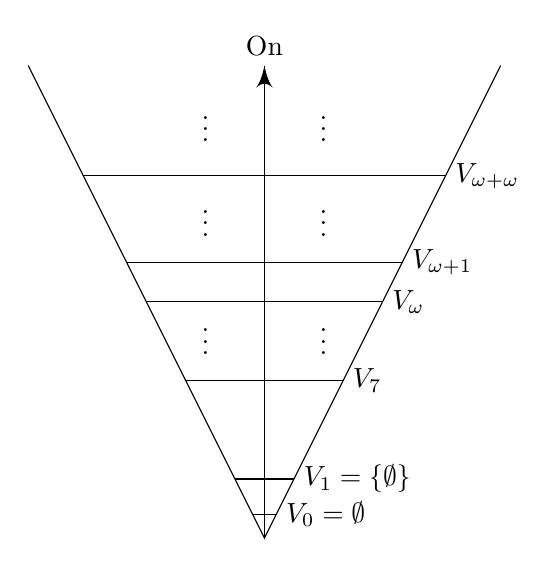
\begin{tikzpicture}
    \draw [->] (0, 0) -- (0, 6) node [above] {On};
    \draw (-3, 6) -- (0, 0) -- (3, 6);
    \draw (-0.15, 0.3) -- (0.15, 0.3) node [right] {$V_0 = \emptyset$};
    \draw (-0.375, 0.75) -- (0.375, 0.75) node [right] {$V_1 = \{\emptyset\}$};
    \draw (-1, 2) -- (1, 2) node [right] {$V_7$};
    \node at (-0.75, 2.6) {$\vdots$};
    \node at (0.75, 2.6) {$\vdots$};
    \draw (-1.5, 3) -- (1.5, 3) node [right] {$V_\omega$};
    \draw (-1.75, 3.5) -- (1.75, 3.5) node [right] {$V_{\omega + 1}$};
    \node at (-0.75, 4.1) {$\vdots$};
    \node at (0.75, 4.1) {$\vdots$};
    \draw (-2.3, 4.6) -- (2.3, 4.6) node [right] {$V_{\omega + \omega}$};
    \node at (-0.75, 5.3) {$\vdots$};
    \node at (0.75, 5.3) {$\vdots$};
  \end{tikzpicture}
\end{center}
Note that by definition, we have $x\subseteq V_\alpha \Leftrightarrow x\in V_{\alpha + 1}$.

We would like every $x$ to be in some $V_\alpha$, and that is indeed true. We prove this though a series of lemmas:

\begin{lemma}
  Each $V_\alpha$ is transitive.
\end{lemma}

\begin{proof}
  Since we define $V_\alpha$ by recursion, it is sensible to prove this by induction:

  By induction on $\alpha$:
  \begin{enumerate}
    \item Zero: $V_0 = \emptyset$ is transitive.
    \item Successors: If $x$ is transitive, then so is $\P(x)$: given $y\in z\in \P(x)$, we want to show that $y\in \P(x)$. Since $y$ is in a member of $\P(x)$, ie. a subset of $x$, we must have $y\in x$. So $y\subseteq x$ since $x$ is transitive. So $y\in \P(x)$.
    \item Limits: Any union of transitive sets is transitive.
  \end{enumerate}
\end{proof}

\begin{lemma}
  If $\alpha \leq \beta$, then $V_\alpha \subseteq V_\beta$.
\end{lemma}

\begin{proof}
  Fix $\alpha$, and induct on $\beta$.
  \begin{enumerate}
    \item $\beta = \alpha$: trivial
    \item Successors: $V_{\beta^+}\subseteq V_\beta$ since $x\subseteq \P(x)$ for transitive $x$. So $V_\alpha \subseteq V_\beta \Rightarrow V_\alpha \subseteq V_{\beta^+}$.
    \item Limits: Trivial by definition
  \end{enumerate}
\end{proof}

Finally we are ready for:
\begin{thm}
  Every $x$ belongs to some $V_\alpha$. Intuitively, we want to say
  \[
    V = \bigcup_{\alpha \in \mathrm{On}} V_\alpha,
  \]
\end{thm}
We'll need some terminology to start with. If $x\subseteq V_\alpha$ for some $\alpha$, then there is a least $\alpha$ with $x\subseteq V_\alpha$. We call this the \emph{rank} of $x$.

For example, $\rank(\emptyset) = 0$, $\rank(\{\emptyset\}) = 1$. Also $\rank(\omega) = \omega$. In fact, $\rank(\alpha) = \alpha$ for all $\alpha\in \mathrm{On}$.

Note that we want the least $\alpha$ such that $x\subseteq V_\alpha$, \emph{not} $x\in V_\alpha$.

\begin{proof}
  We'll show that $(\forall x)(\exists \alpha)(x\in V_\alpha)$ by $\in$-induction on $x$.

  So we are allowed to assume that for each $y\in x$, we have $y\subseteq V_\alpha$ for some $\alpha$. So $y\subseteq V_{\rank(y)}$, or $y\in V_{\rank(y) + 1}$.

  Let $\alpha = \sup\{(\rank(y)^+: y\in x\}$. Then $y\in V_\alpha$ for every $y\in x$. So $x\subseteq V_\alpha$.
\end{proof}

Our definition of rank is easy to get wrong --- it is easy to be off by of 1. So the official definition is
\begin{defi}[Rank]
  The \emph{rank} of a set $x$ is defined recursively by
  \[
    \rank(x) = \sup\{(\rank y)^+ : y\in x\}.
  \]
\end{defi}

Then the initial definition we had is now a proposition.
\begin{prop}
  $\rank(x)$ is the first $\alpha$ such that $x\subseteq V_\alpha$.
\end{prop}

\section{Cardinals}
In this chapter, we will look at the ``sizes'' of (infinite) sets (finite sets are boring!). We work in ZFC, since things become really weird without Choice.

Since we will talk about bijections a lot, we will have the following notation:
\begin{notation}
  Write $x\leftrightarrow y$ for $\exists f: f$ is a bijection from $x$ to $y$.
\end{notation}

\subsection{Definitions}
We want to define $\card(x)$ (the \emph{cardinality}, or \emph{size} of $x$) in such a way that $\card(x) = \card(y) \Leftrightarrow x\leftrightarrow y$. We can't define $\card(x) = \{y: y\leftrightarrow x\}$ as it may not be a set. So we want to pick a ``representative'' of the sets that biject with $x$, like how we defined the ordinals.

So why not use the ordinals? By Choice, we know that all $x$ is well-orderable. So $x\leftrightarrow \alpha$ for some $\alpha$. So we define:
\begin{defi}[Cardinality]
  The \emph{cardinality} of a set $x$, written $\card(x)$, is the least ordinal $\alpha$ such that $x\leftrightarrow y$.
\end{defi}
Then we have (trivially) $\card(x) = \card(y) \Leftrightarrow x\leftrightarrow y$.

(What if we don't have Choice, ie. if we are in ZF? This will need a really clever trick, called the \emph{Scott trick}. In our universe of ZF, there is a huge of blob of things that biject with $x$. We cannot take the whole blob (it won't be a set), or pick one of them (requires Choice). So we ``chop off'' the blob at fixed, determined point, so we are left with a set.

Define the essential rank of $x$ to be the least rank of all $y$ such that $y\leftrightarrow x$. Then set $\card (x) = \{y\in V_{\mathrm{essrank}(x)^+}: y\leftrightarrow x\}$.)

So what cardinals are there? Clearly we have $1, 2, 3, \cdots$. What else?

\begin{defi}[Initial ordinal]
  We say an ordinal $\alpha$ is \emph{initial} if
  \[
    (\forall \beta < \alpha)(\neg \beta \leftrightarrow \alpha),
  \]
  ie. it is the smallest ordinal of that cardinality.
\end{defi}

Then $0, 1, 2, 3, \cdots, \omega, \omega_1, \gamma(X)$ for any $X$ are all initial. However, $\omega^\omega$ is not initial, as it bijects with $\omega$ (both are countable).

Can we find them all? Yes!
\begin{defi}[Omega ordinals]
  We define $\omega_\alpha$ for each $\alpha \in \mathrm{On}$ by
  \begin{enumerate}
    \item $\omega_0 = \omega$;
    \item $\omega_{\alpha + 1} = \gamma(\omega_\alpha)$;
    \item $\omega_\lambda = \sup\{\omega_\alpha: \alpha < \lambda\}$ for non-zero limit $\lambda$.
  \end{enumerate}
\end{defi}
It is easy induction to show that each $\omega_\alpha$ is initial. We can also show that every initial $\delta$ (for $\delta \geq \omega$) is an $\omega_\alpha$. We know that the $\omega_\alpha$ are unbounded since, say $\omega_\alpha \geq \alpha$ for all $\alpha$. So there is a least $\alpha$ with $\omega_\alpha \geq \delta$.

If $\alpha$ is a successor, then let $\alpha = \beta^+$. Then $\omega_\beta < \delta \leq \omega_\alpha$. But there is no initial ordinal between $\omega_\beta$ and $\omega_\alpha = \gamma(\omega_\beta)$, since $\gamma(X)$ is defined as the \emph{least} ordinal that does not biject with $X$. So we must have $\delta = \omega_\alpha$.

If $\alpha$ is a limit, then since $\omega_\alpha$ is defined as a supremum, by definition we cannot have $\delta < \omega_\alpha$, or else there is some $\beta < \alpha$ with $\delta < \omega_\beta$. So $\omega_\alpha = \delta$ as well.

\begin{defi}[Aleph number]
  Write $\aleph_\alpha$ (``aleph-$\alpha$'') for $\card(\omega_\alpha)$.
\end{defi}

Then from the argument above, we have
\begin{thm}
  The $\aleph_\alpha$ are the cardinals of all infinite sets (or, in ZF, the cardinals of all infinite well-orderable sets). For example, $\card(\omega) = \aleph_0$, $\card \omega_1 = \aleph_1$.
\end{thm}

We will use lower case letters to denote cardinalities and upper case for the sets with that cardinality. eg. $\card(N) = n$.

\begin{defi}[Cardinal (in)equality]
  For cardinals $n$ and $m$, write $m \leq n$ if $M$ injects into $N$, where $\card M = m, \card N = n$. This clearly does not depend on $M$ and $N$.

  So $m \leq n$ and $n\leq m$ implies $n = m$ by Schr\"oder-Bernstein. Write $m < n$ if $m \leq n$ by $m\not = n$.
\end{defi}

\begin{eg}
  $\card(\P(\omega)) > \card(\omega)$.
\end{eg}

This $\leq$ is a partial order. Moreover, it is a total order (assuming AC).

\subsection{Cardinal arithmetic}
\begin{defi}[Cardianl addition, multiplication and exponentiation]
  For cardinals $m, n$, write $m + n$ for $\card(M\sqcup N)$; $mn$ for $\card(M\times N)$; and $m^n$ for $\card(M^N)$, where $M^N = \{f: f\text{ is a function }N\to M\}$. Note that this coincides with our usual definition of $X^n$ for finite $n$.
\end{defi}

\begin{eg}
  $\R \leftrightarrow \P(\omega) \leftrightarrow 2^\omega$. So $\card(\R) = \card(\P_\omega) = 2^{\aleph_0}$.
\end{eg}

Similarly, define
\[
  \sum_{i \in I} m_i = \card\left(\bigsqcup_{i\in I} M_i\right).
\]

\begin{eg}
  How many sequences of reals are there? A real sequence is a function from $\omega \to \R$. We have
  \[
    \card(\R^\omega) = (2^{\aleph_0})^{\aleph_0} = 2^{\aleph_0 \times \aleph_0} = 2^{\aleph_0} = \card(\R)
  \]
\end{eg}
Note that we used facts like
\begin{prop}\leavevmode
  \begin{enumerate}
    \item $m + n = n + m$ since $N\sqcup M \leftrightarrow N\sqcup N$ with the obvious bijection.
    \item $mn = nm$ using the obvious bijection
    \item $(m^n)^p = m^{np}$ as $(M^N)^P \leftrightarrow M^{N\times P}$ since both objects take in a $P$ and an $N$ and returns an $M$.
  \end{enumerate}
\end{prop}
It is important to note that cardinal exponentiation is different from ordinal exponentiation. For example, $\omega^\omega$ (ordinal exponentiation) is countable, but $\aleph_0^{\aleph_0} \geq 2^{\aleph_0} > \aleph_0$ (cardinal exponentiation).

From IA Numbers and sets, we know that $\aleph_0 \aleph_0 = \aleph_0$. What about $\aleph_1 \aleph_1$? Or $\aleph_3 \aleph_0$?

It turns out that cardinal sums and multiplications are utterly boring:
\begin{thm}
  For every ordinal $\alpha$,
  \[
    \aleph_\alpha \aleph_\alpha = \aleph_\alpha.
  \]
  This is the best we could ever ask for. What can be simpler?
\end{thm}

\begin{proof}
  Since the Alephs are defined by induction, it makes sense to prove it by induction.

  In the following proof, there is a small part that doesn't work nicely with $\alpha = 0$. But $\alpha = 0$ case (ie $\aleph_0\aleph_0 = \aleph_0$) is already done. So assume $\alpha \not= 0$.

  Induct on $\alpha$. We want $\omega_\alpha \times \omega_\alpha$ to biject with $\omega_\alpha$, ie. well-order $\omega_\alpha \times \omega_\alpha$ to an ordering of length $\omega_\alpha$.

  Using the ordinal product clearly doesn't work. The ordinal product counts the product in rows, so we have many copies of $\omega_\alpha$. When we proved $\aleph_0\aleph_0 = \aleph_0$, we counted them diagonally. But counting diagonally here doesn't look very nice, since we will have to ``jump over'' infinities. Instead, we count in squares
  \begin{center}
    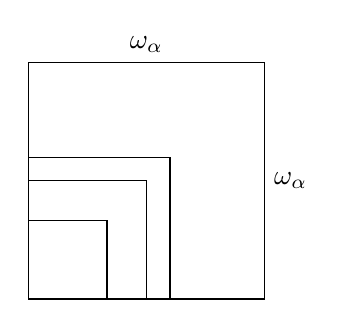
\begin{tikzpicture}
      \draw rectangle (3, 3);
      \node at (1.5, 3) [above] {$\omega_\alpha$};
      \node at (3, 1.5) [right] {$\omega_\alpha$};
      \draw (0, 1) -- (1, 1) -- (1, 0);
      \draw (0, 1.5) -- (1.5, 1.5) -- (1.5, 0);
      \draw (0, 1.8) -- (1.8, 1.8) -- (1.8, 0);
    \end{tikzpicture}
  \end{center}
  We set $(x, y) < (x', y')$ if \emph{either} $\max(x, y) < \max(x', y')$ (this says that $(x', y')$ is in a bigger square), \emph{or}, (say $\max(x, y) = \max(x', y') = \beta$ and $y' = \beta, y < \beta$ or $x = x' = \beta, y < y'$ or $y = y' = \beta, x < x'$) (nonsense used to order things in the same square --- utterly unimportant).

  How do we show that this has order type $\omega_\alpha$? We show that any initial segment has order type $ < \omega_\alpha$.

  For any proper initial segment $I_{(x, y)}$, we have
  \[
    I_{(x, y)} \subseteq \beta\times \beta
  \]
  for some $\beta < \omega_\alpha$, since $\omega_\alpha$ is a limit, with wlog $\beta$ infinite. So
  \[
    \beta\times \beta \leftrightarrow \beta
  \]
  by induction hypothesis (their cardinality is less that $\omega_\alpha$). So
  \[
    \card(\beta\times \beta) < \card(\omega_\alpha).
  \]
  Hence $I_{(x, y)}$ has order type $ < \omega_\alpha$. Thus the order type of our well-order is $\leq \omega_\alpha$. So $\omega_\alpha \times \omega_\alpha$ injects into $\omega_\alpha$. Since trivially $\omega_\alpha$ injects into $\omega_\alpha \times \omega_\alpha$, we have $\omega_\alpha \times \omega_\alpha \leftrightarrow \omega_\alpha$.
\end{proof}
So why did we say cardinal arithmetic is boring? We have
\begin{cor}
  Let $\alpha \leq \beta$. Then
  \[
    \aleph_\alpha + \aleph_\beta = \aleph_\alpha\aleph_\beta = \aleph_\beta.
  \]
\end{cor}

\begin{proof}
  \[
    \aleph_\beta \leq \aleph_\alpha + \aleph_\beta \leq \aleph_\beta + \aleph_\beta = 2\aleph_\beta \leq \aleph_\beta\times \aleph_\beta = \aleph_\beta,
  \]
  So done
\end{proof}

\begin{eg}
  $X\sqcup X$ bijects with $X$, for infinite $X$ (in ZFC).
\end{eg}

However, cardinal exponentiation is \emph{very hard}. For example, is $2^{\aleph_0} = \aleph_1$? This is the continuum hypothesis, and cannot be proved or disproved in ZFC!

Even today, not all implications among values of $\aleph_\alpha^{\aleph_\beta}$ are known, ie. we don't know whether they are true, false or independent!
\section{Incompleteness*}
The big goal of this (non-examinable) chapter is to show that PA is incomplete, ie. there is a sentence $p$ such that $\mathrm{PA}\not\vdash p$ and $\mathrm{PA}\not\vdash \neg p$.

The strategy is to find a $p$ that is true in $\N$, but $\mathrm{PA}\not\vdash p$.

Here we say ``true'' to mean ``true in $\N$'', and ``provable'' to mean ``PA proves it''.

The idea is to find a $p$ that says ``I am not provable''. More precisely, we want a $p$ such that $p$ is true if and only if $p$ is not provable. We are then done: $p$ must be true, since if $p$ were false, then it is provable, ie. $\mathrm{PA}\vdash p$. So $p$ holds in every model of PA, and in particular, $p$ holds in $\N$. Contradiction. So $p$ is true. So $p$ is not provable.

We'll have to ``code'' formulae, proofs etc. inside PA, ie. as numbers. But this doesn't seem possible --- it seems like, in any format, ``$p$ is not provable'' must be longer than $p$. So $p$ cannot say ``$p$ is not provable``!

So be prepared for some magic to come up in the middle for the proof!

\subsection*{Definability}
We first start with some notions of definability.

\begin{defi}[Definability]
  A subset $S\subseteq \N$ is \emph{definable} if there is a formula $p$ with one free variable such that
  \[
    \forall m\in \N:\; m\in S \Leftrightarrow p(m)\text{ holds}.
  \]
  Similarly, $f: \N \to \N$ is \emph{definable} if there exists a formula $p(x, y)$ such that
  \[
    \forall m, n\in \N:\; f(m) = n \Leftrightarrow p(m, n)\text{ holds}.
  \]
\end{defi}

\begin{eg}
  The set of primes is definable: $p(x)$ is
  \[
    x\not = 1 \wedge (\forall y)(\forall z)(yz = x \Rightarrow (y = 1\vee z = 1)).
  \]
  We can say ``$m$ is prime'' is definable.

  How about powers of $2$? We don't have exponentiation here. What can we do? We can take $p(x)$ to be
  \[
    (\forall y)((y\text{ is prime}\wedge y \mid x) \Rightarrow y = 2),
  \]
  where $2$ is a shorthand for $s(s(0))$, and $y\mid x$ is a shorthand for $(\exists z)(yz = x)$. So this is also definable.

  The function $m\mapsto m^2$ is also definable: take $p(x, y)$ to be $yy = x$.
\end{eg}

Here we will assume:
\begin{fact}
  Any function given by an algorithm is definable.
\end{fact}
Proof will not be given here. See, eg, PTJ's book for detailed proof.

\begin{eg}
  $m\mapsto 2^m$ is definable.
\end{eg}

\subsection*{Coding}
Our language has 12 symbols: $s, 0, \times, +, \bot, \Rightarrow, (, ), =, x, ', \forall$ (where the variables are now called $x, x', x'', x'''$.

We assign values to them, say $v(s) = 1, v(0) = 2, \cdots, v(\forall) = 12$. To code a formula, we can take
\[
  2^{v(\text{first symbol})}\cdot 3^{v(\text{second symbol})}\cdots (n\text{th prime})^{v(n\text{th symbol})}.
\]
For example, $(\forall x)(x = x)$ is coded as
\[
  2^7 3^{12}5^{10}7^8 11^7 13^{10}17^9 23^8.
\]
Not every $m$ codes a formula, eg. $2^7 3^{12}5^{10}$ is translated to $(\forall x$, which is clearly nonsense. Similarly, $2^7 7^3$ or $2^{100}$ can't even be translated at all.

However, ``$m$ codes a formula'' is definable, as there is an algorithm that checks that.

Write $S_m$ for the formula coded by $m$ (and set $S_m$ to be ``$\bot$'' if $m$ does not code a formula). Similarly, write $c(p)$ for the code of $p$.

Given a finite sequence $p_1, \cdots p_n$ for formulae, code it as
\[
  2^{c(p_1)}3^{c(p_2)}\cdots (n\text{th prime})^{c(p_n)}.
\]
Alternatively, we can add a separator character to our 12 symbols and concatenate the sequence of formulae with the separator character.

Now, ``$m$ codes an axiom (either logical or axiom of PA)'' is definable, as there exists an algorithm to check it. For example, an instance of the first logical axiom can be validated by the following regex:
\[
  \verb/^\([s0()=x'\+/\mathtt{\times\bot\Rightarrow\forall}\verb/]+\)/\mathtt{\Rightarrow}\verb/([s0()=x'\+/\mathtt{\times\bot\Rightarrow\forall}\verb/]+/\Rightarrow\verb/\1)$/
\]
(after translating to a sentence and verifying it is a valid logical formula)

Also,
\begin{center}
  $\phi(\ell, m, n) = $``$S_n$ obtained from $S_\ell$, $S_m$ via MP''
\end{center}
is definable, and similarly for generalization.

So
\[
  \Theta(m, n) =\text{``}n\text{ codes a proof of }S_m\text{''}
\]
is definable.

Thus
\[
  \Psi(m) = \text{``}S_m\text{ is provable''}
\]
is definable as
\[
  \Psi(m) \Leftrightarrow (\exists n)\Theta(m, n).
\]
So far, everything is rather boring. We all \emph{know} that strings of symbols can be coded into numbers --- that's what computers do!

\subsection*{Clever bit}
Consider the statement $\chi(m)$ that states
\begin{center}
  ``$m$ codes a formula $S_m$ with one free variable, and $S_m(m)$ is not provable.''
\end{center}
This is clearly definable. Suppose this is defined by $p$. So
\[
  \chi(n) \Leftrightarrow p[n/x]
\]
Suppose $c(p) = N$. Then $\chi(N)$ asserts
\begin{center}
  ``$N$ codes a formula $S_N$ with one free variable and $S_N(N)$ is not provable.''
\end{center}
But we already know that $N$ codes the formula $\chi$. So $\chi(N)$ asserts that $\chi(N)$ is not provable.

So
\begin{thm}[G\"odel's incompleteness theorem]
  PA is incomplete.
\end{thm}

Maybe that's because PA is rubbish. Could we add some clever axiom $t$ (true in $\N$) to PA, so that PA$\cup \{t\}$ is complete? No! Just run the same proof with ``PA'' replaced by ``PA$\cup \{t\}$'' to show that PA$\cup\{t\}$ is incomplete.

But we can certainly extend PA to a complete theory --- let $T = \{p: p\text{ holds in }\N\}$. What will go wrong in our proof? It can only be because
\begin{thm}
  ``Truth is not definable''

  $T= \{p: p\text{ holds in }\N\}$ is not definable. This officially means
  \[
    \{m: m\text{ codes a member of }T\}
  \]
  is not a definable set.
\end{thm}

Next question: we proved that our clever statement $p$ is true but not provable. Why doesn't this formalize into PA? The answer is, in the proof, we also used the fact that PA has a model, $\N$. By completeness, this means that we used the statement con(PA), ie. the statement that PA is consistent, or
\[
  (\forall m)(m\text{ does not code a proof of }\bot).
\]
With this statement, the proof does formalize to PA. So PA$\cup \{\text{con(PA)}\}\vdash p$. Hence
\begin{thm}
  PA $\not \vdash$ con(PA).
\end{thm}

The same proof works in ZF. So ZF is incomplete and ZF does not prove its own consistency.
\end{document}
